\documentclass[../main.tex]{subfiles}
\begin{document}
\section{Тензоры}
	\subsection{Линейные формы(линейные функционалы). Сопряженное пространство. Ковариантные, контрвариантные преобразования.}
		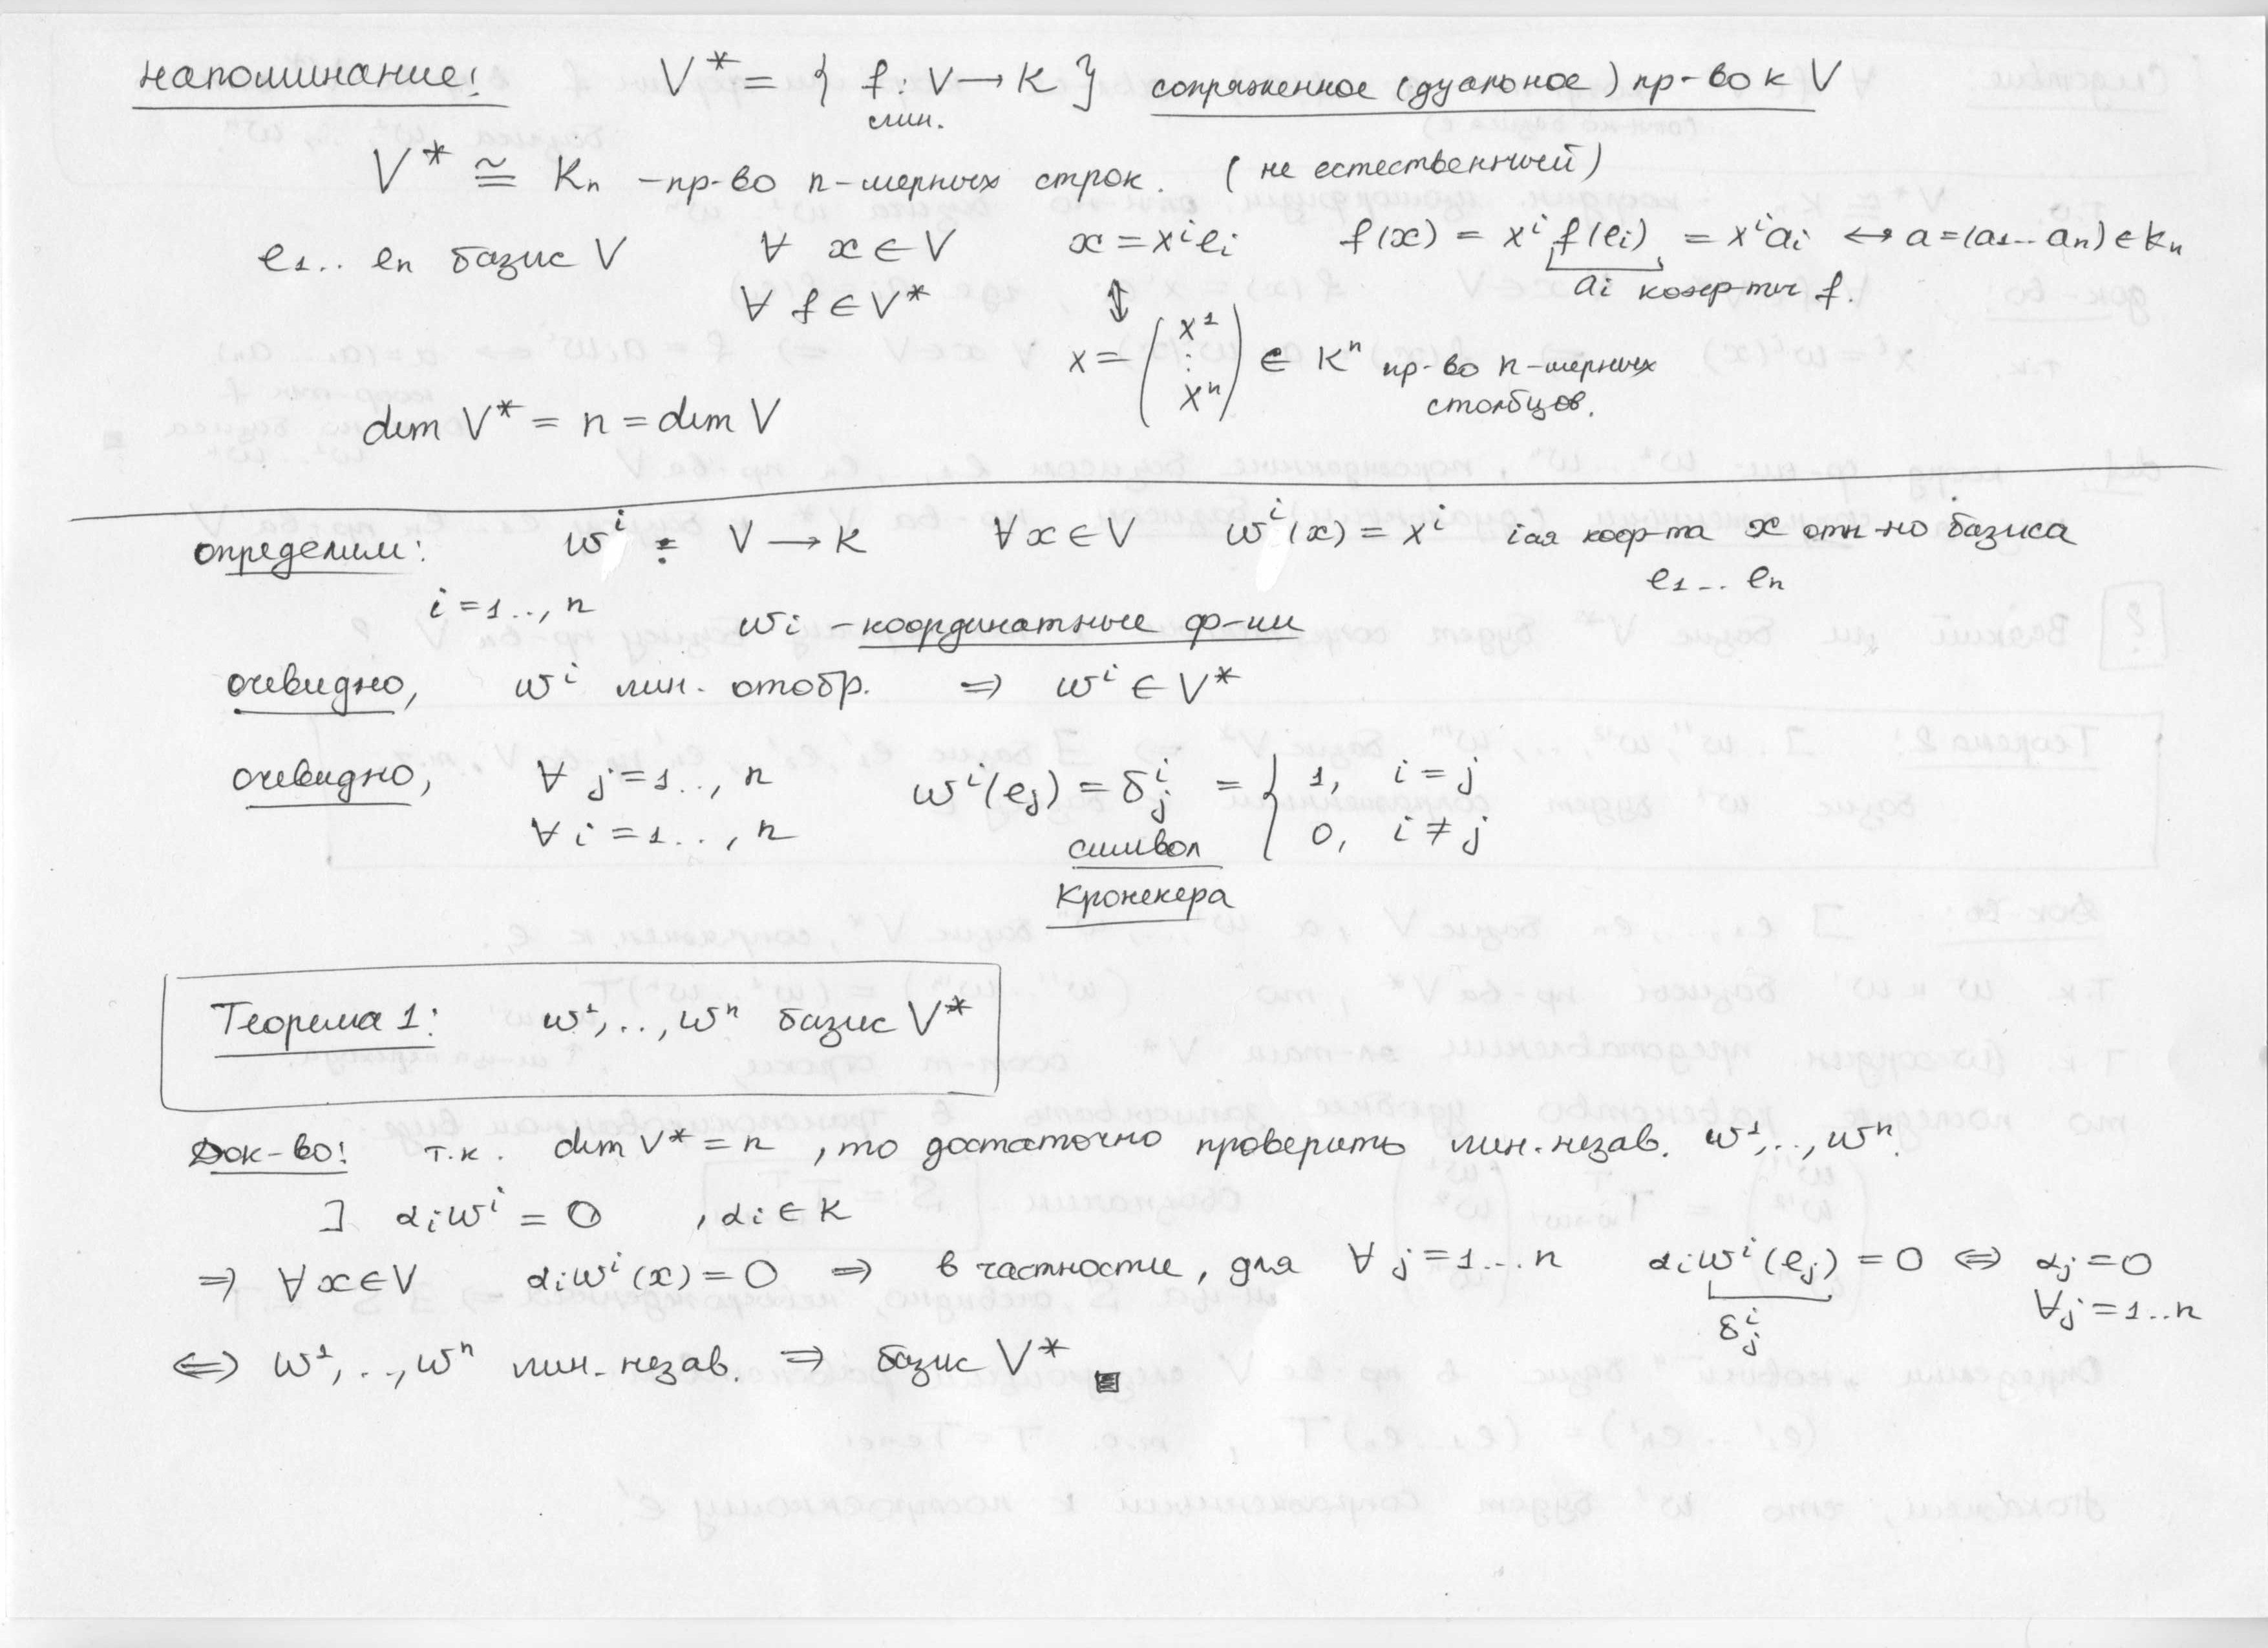
\includegraphics[height=\textheight * 10 / 21, width=\textwidth]{8_1-1}	
		\newline
		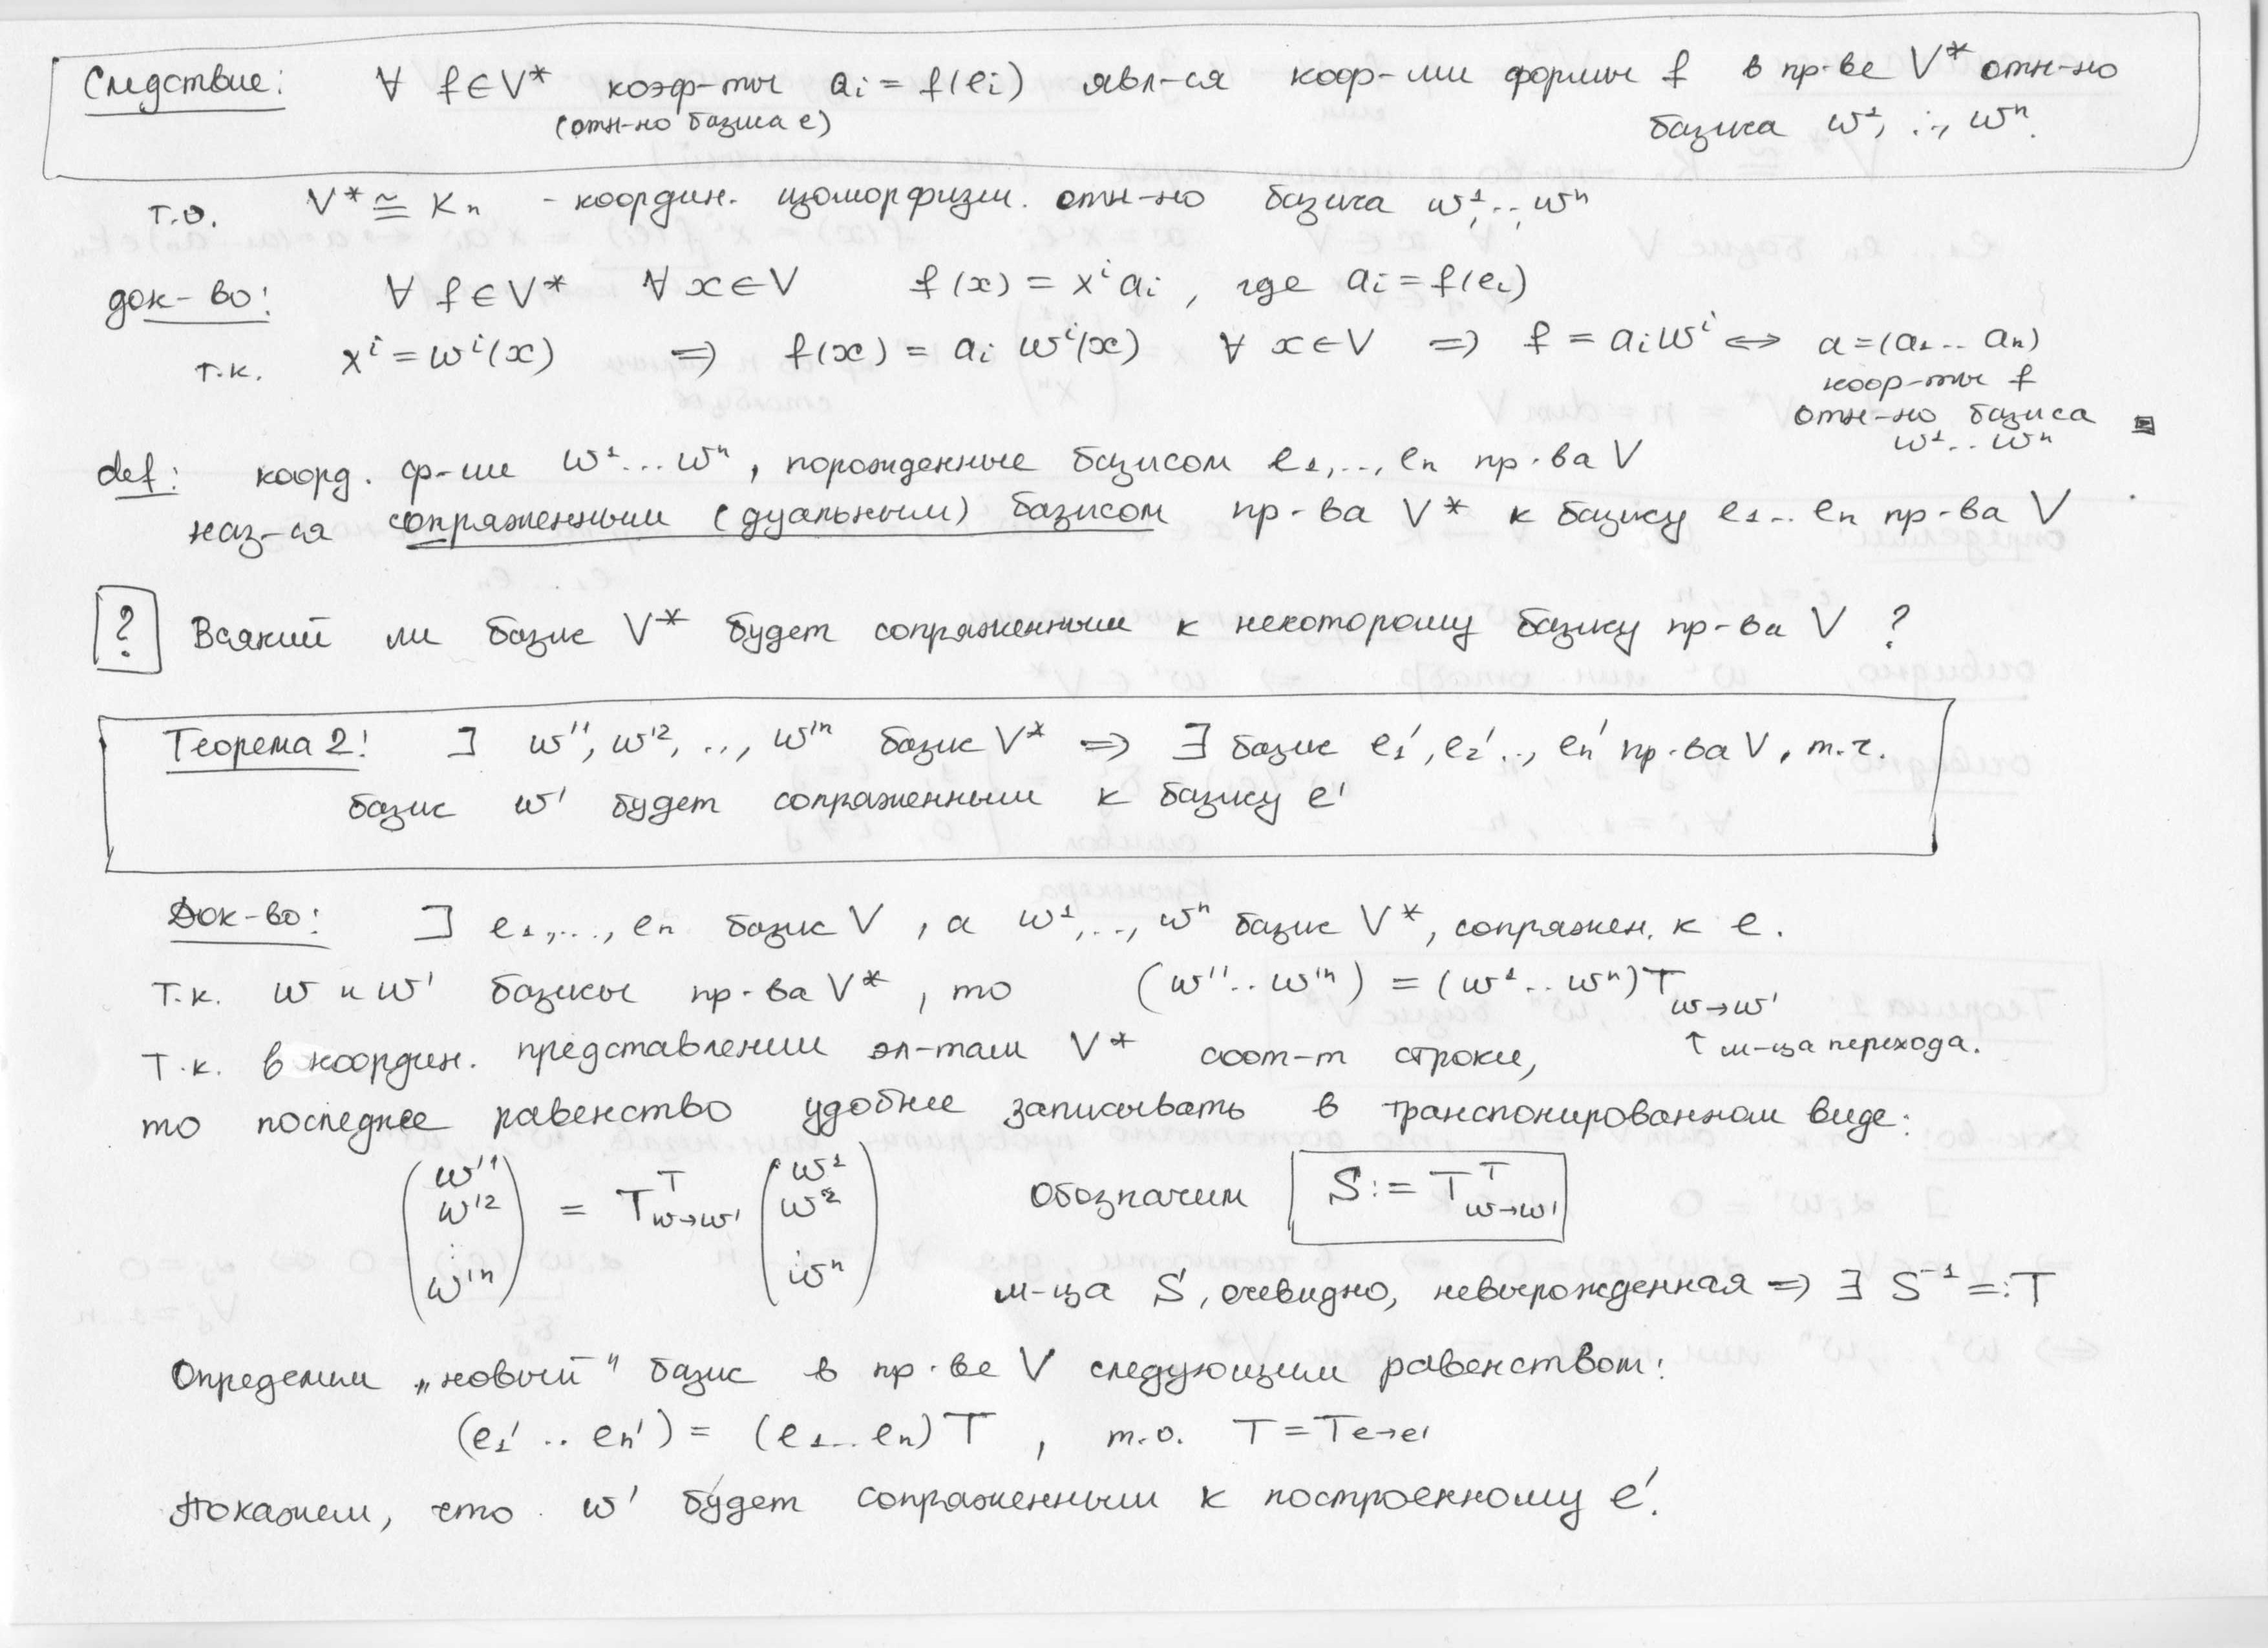
\includegraphics[height=\textheight * 10 / 21, width=\textwidth]{8_1-2}	
		\newline
		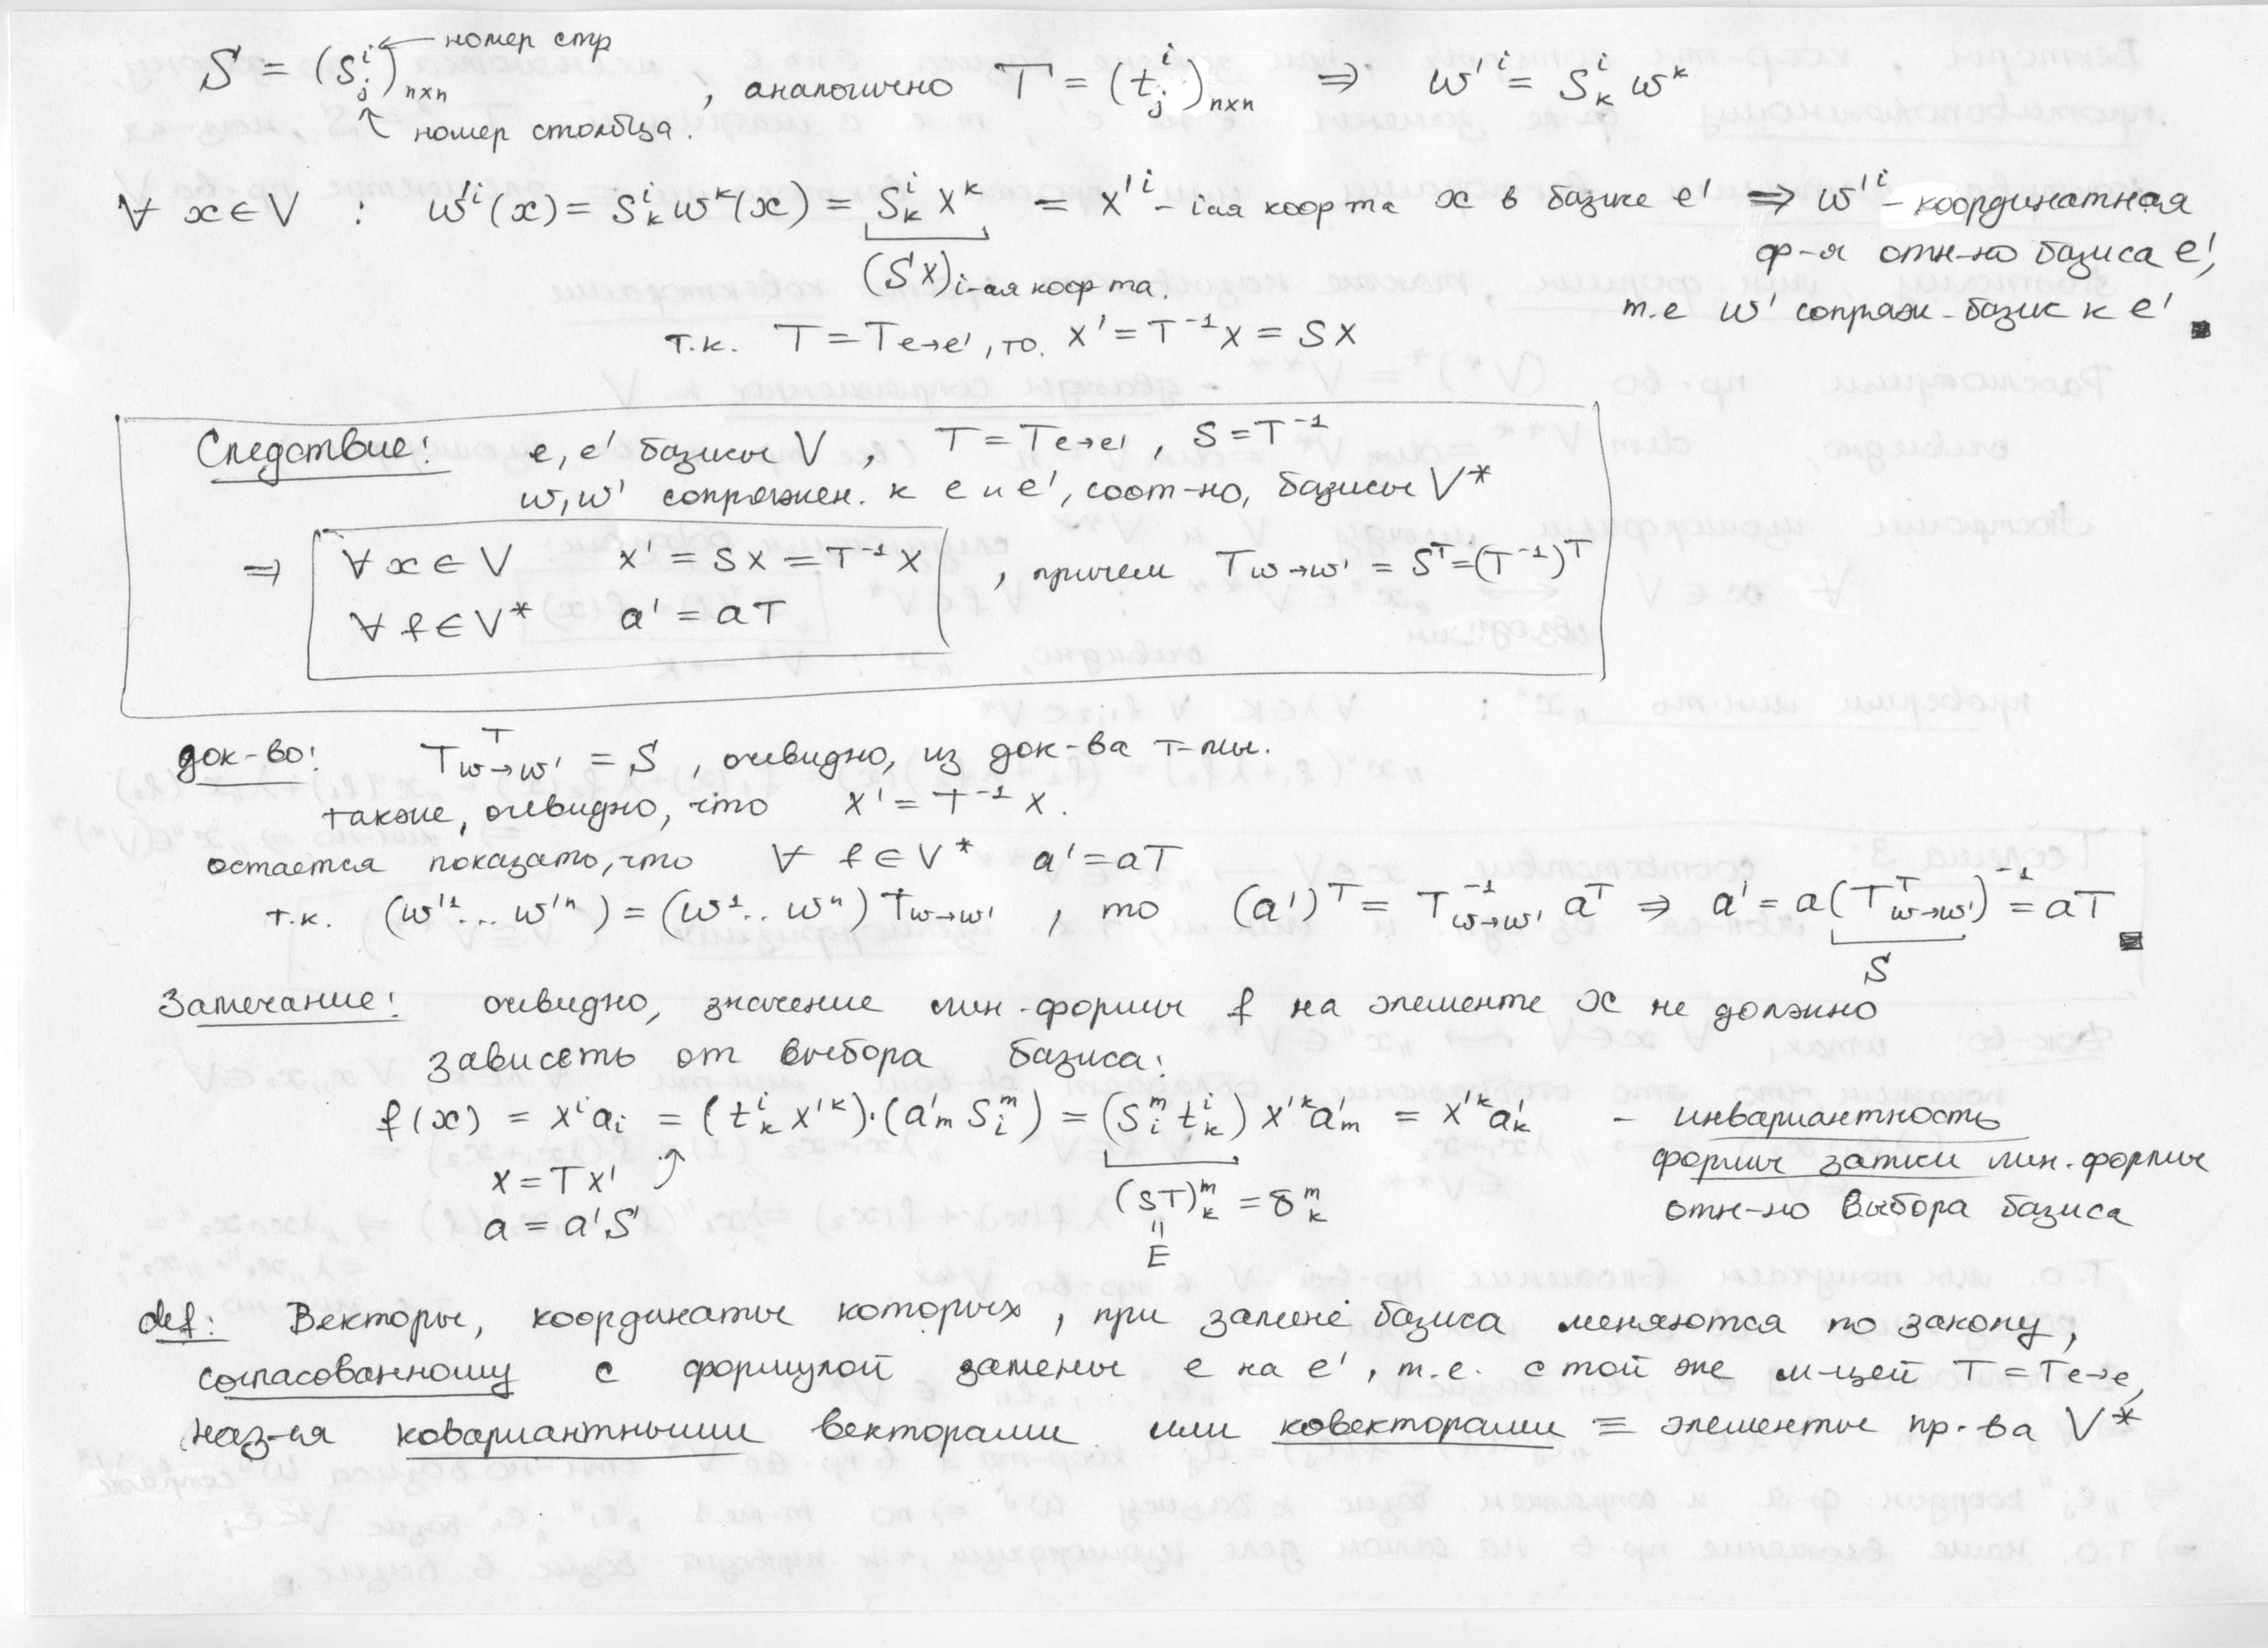
\includegraphics[height=\textheight * 10 / 21, width=\textwidth]{8_1-3}	
		\newline
		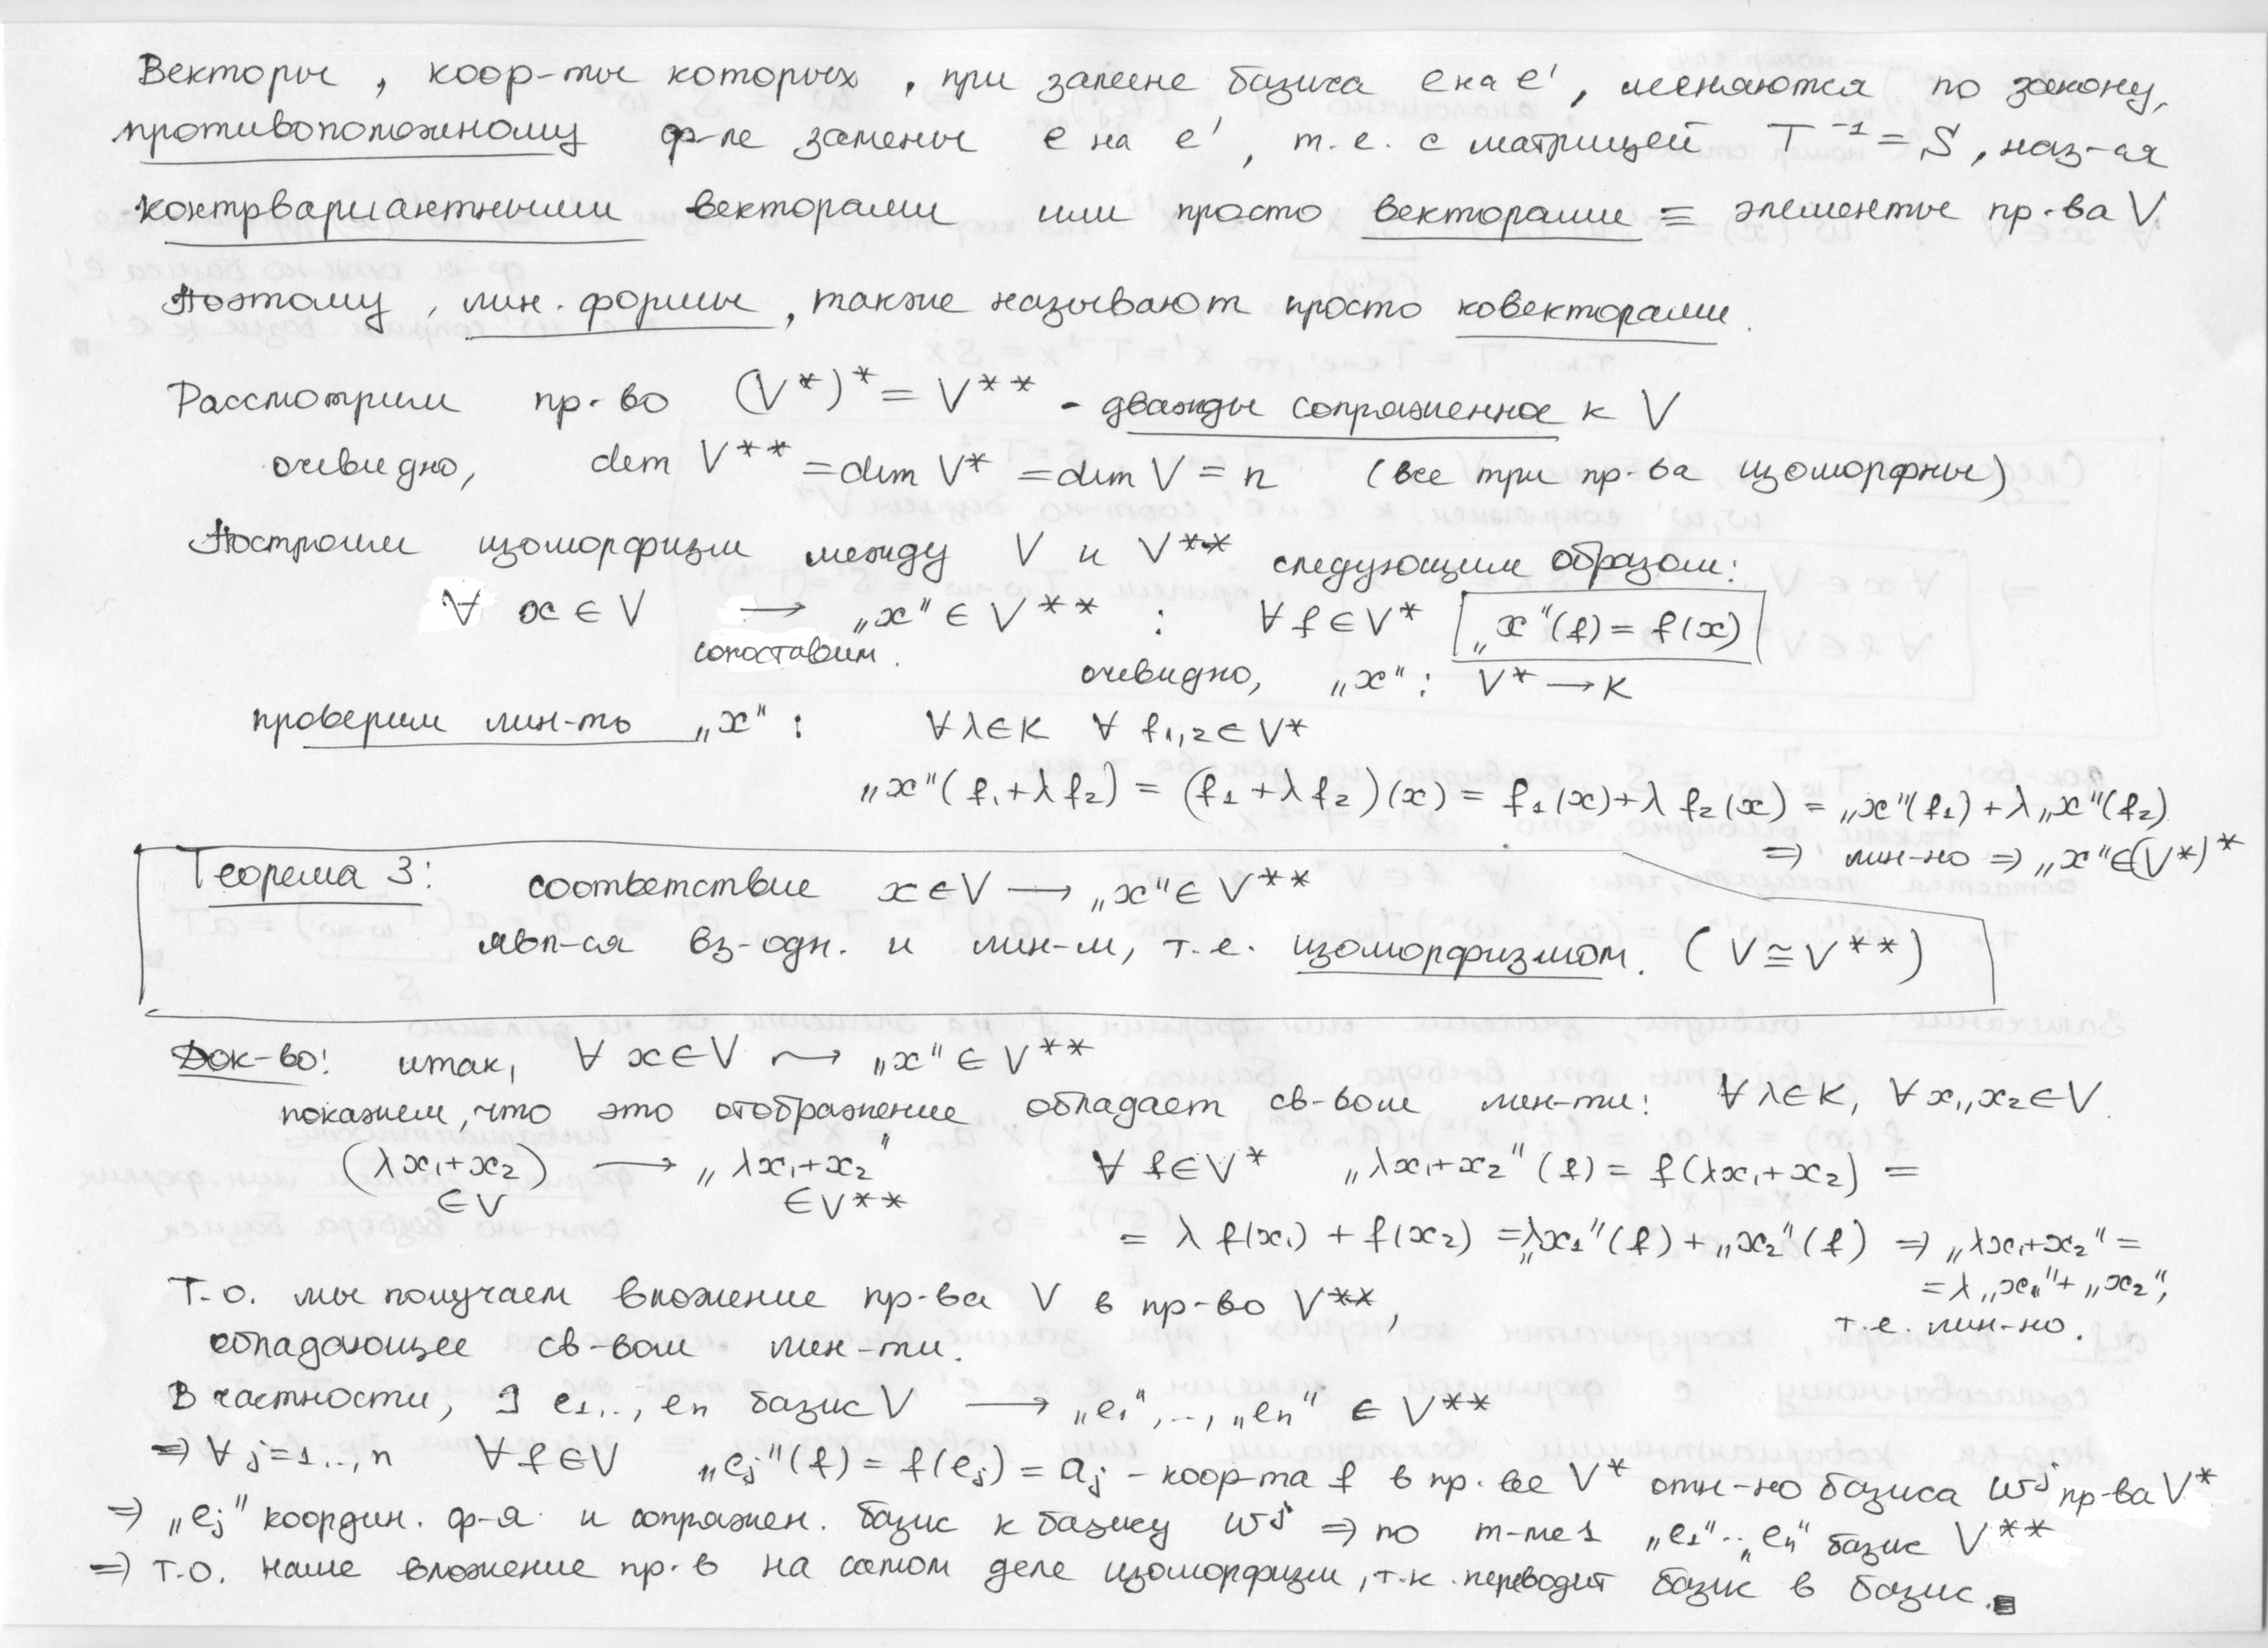
\includegraphics[height=\textheight * 10 / 21, width=\textwidth]{8_1-4}	
		\newline
		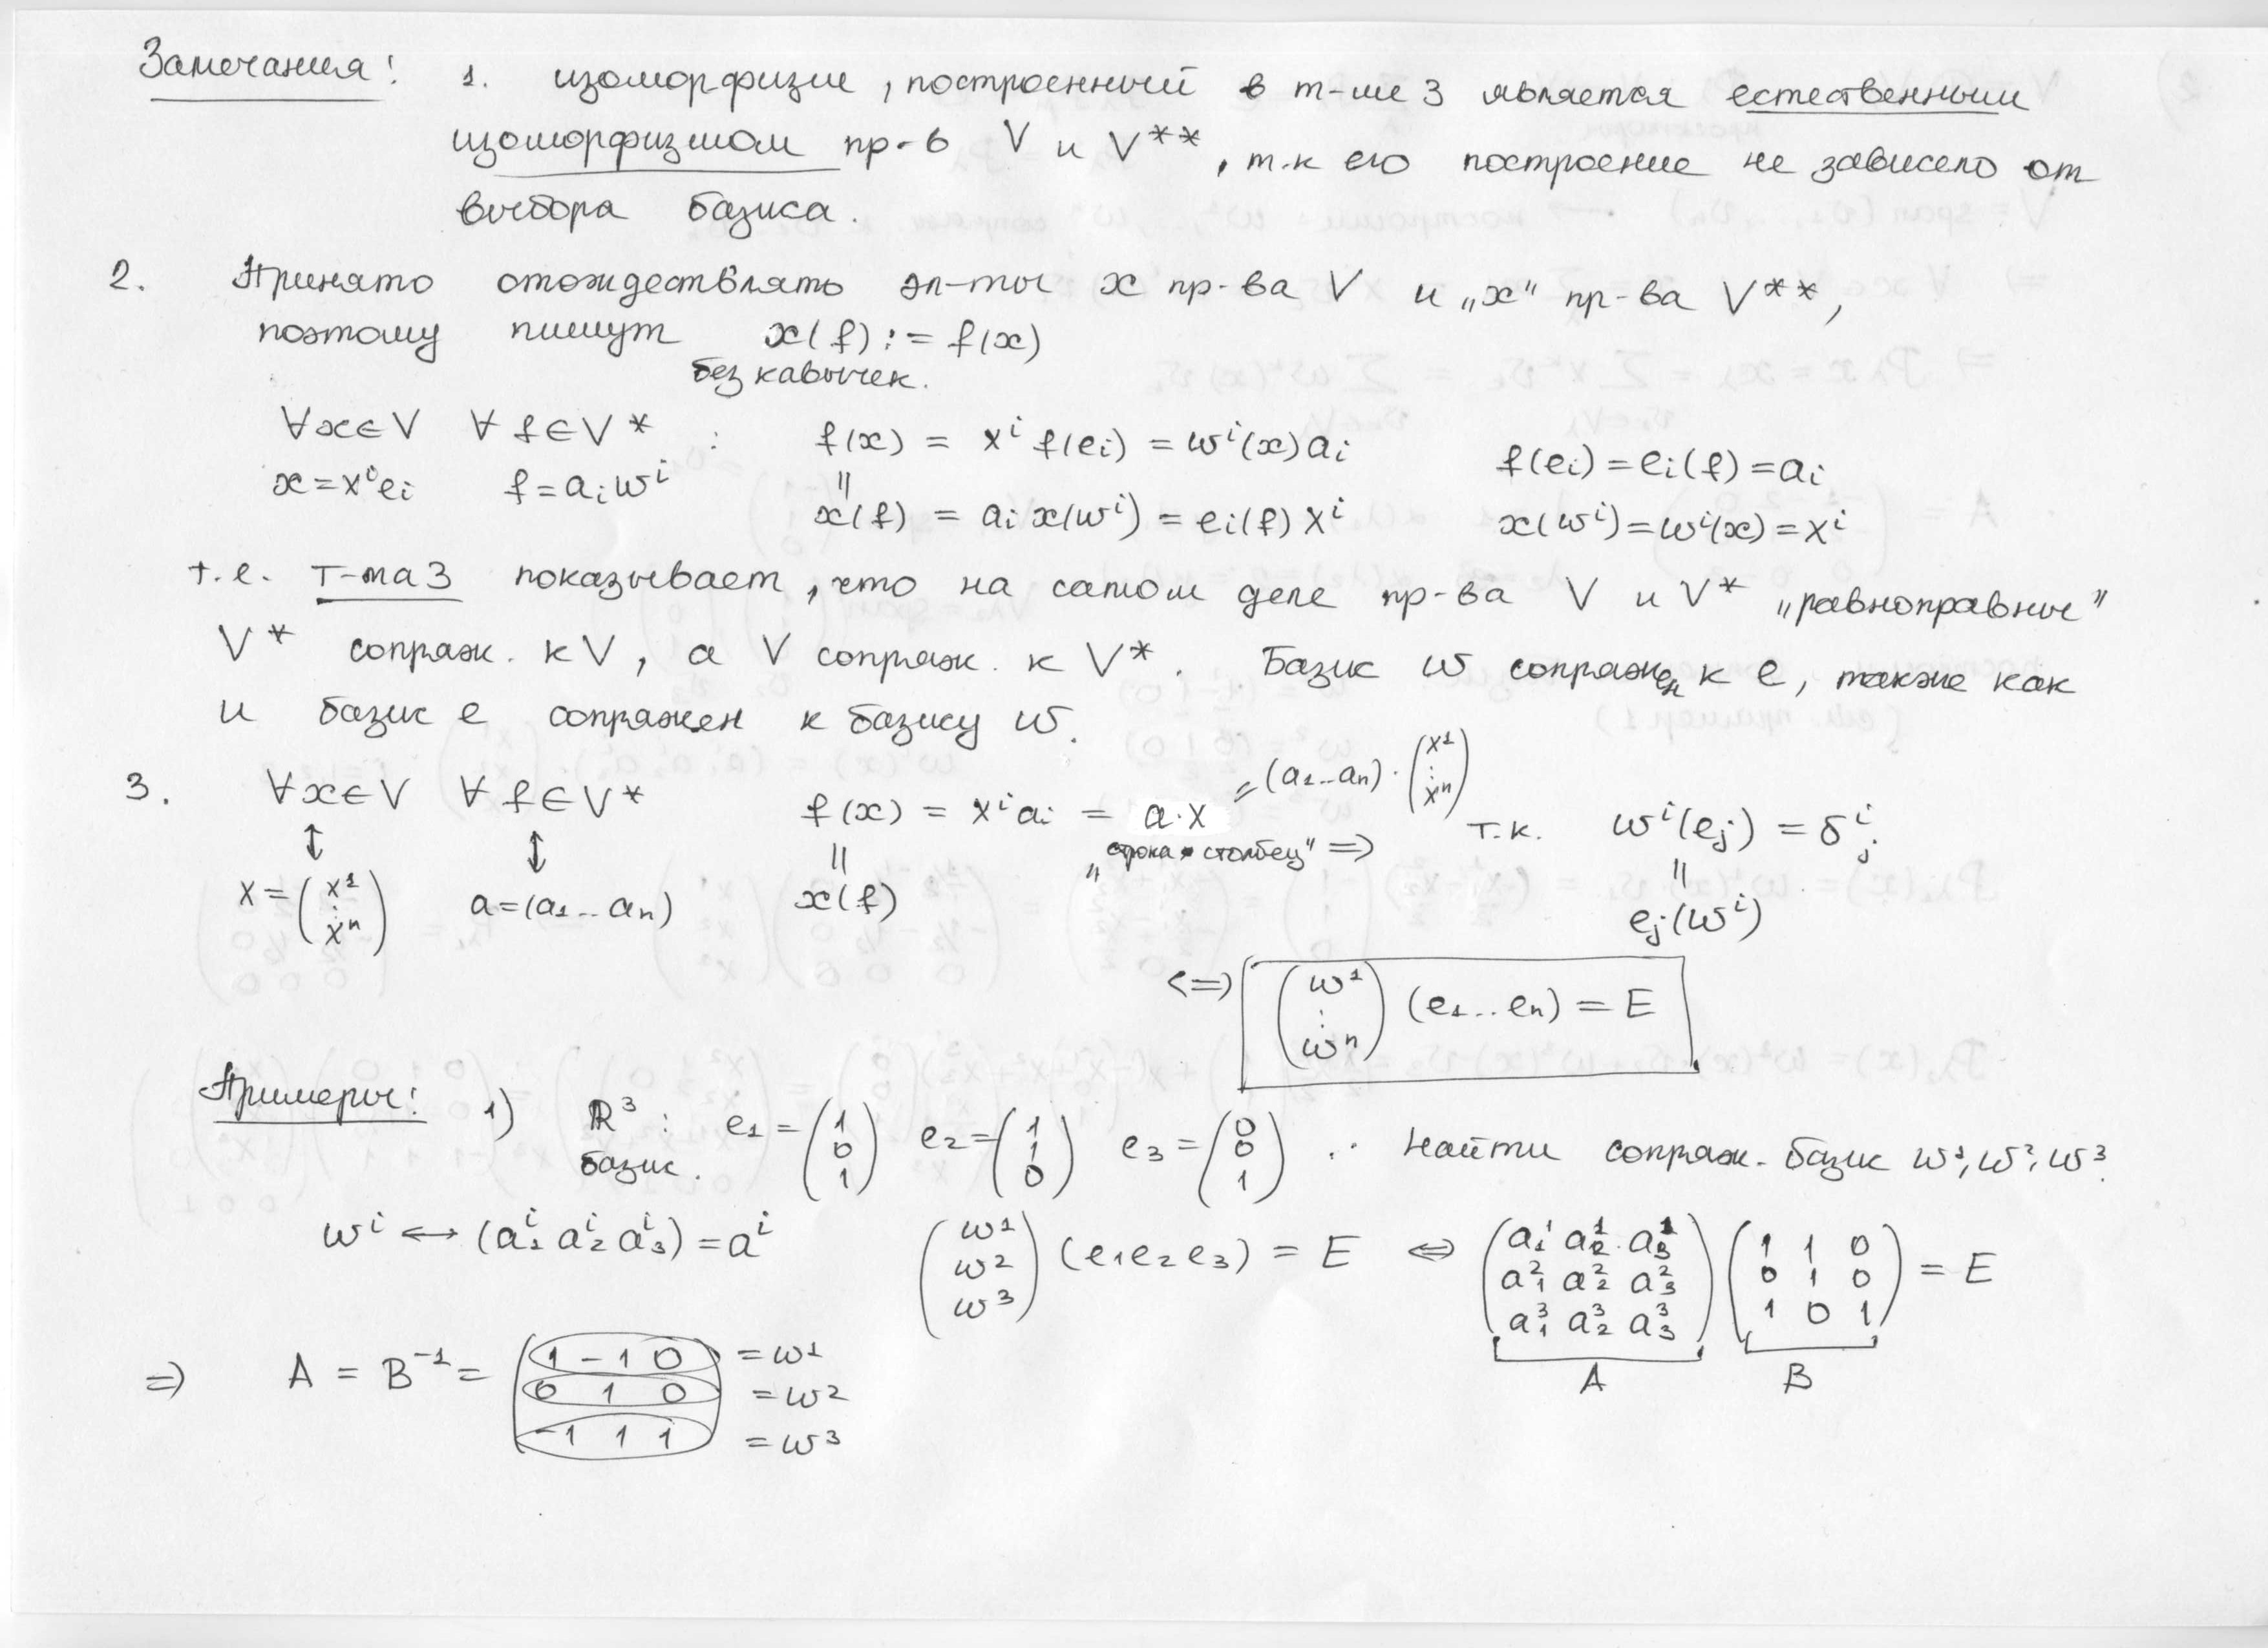
\includegraphics[height=\textheight * 10 / 21, width=\textwidth]{8_1-5}	
		\newline
		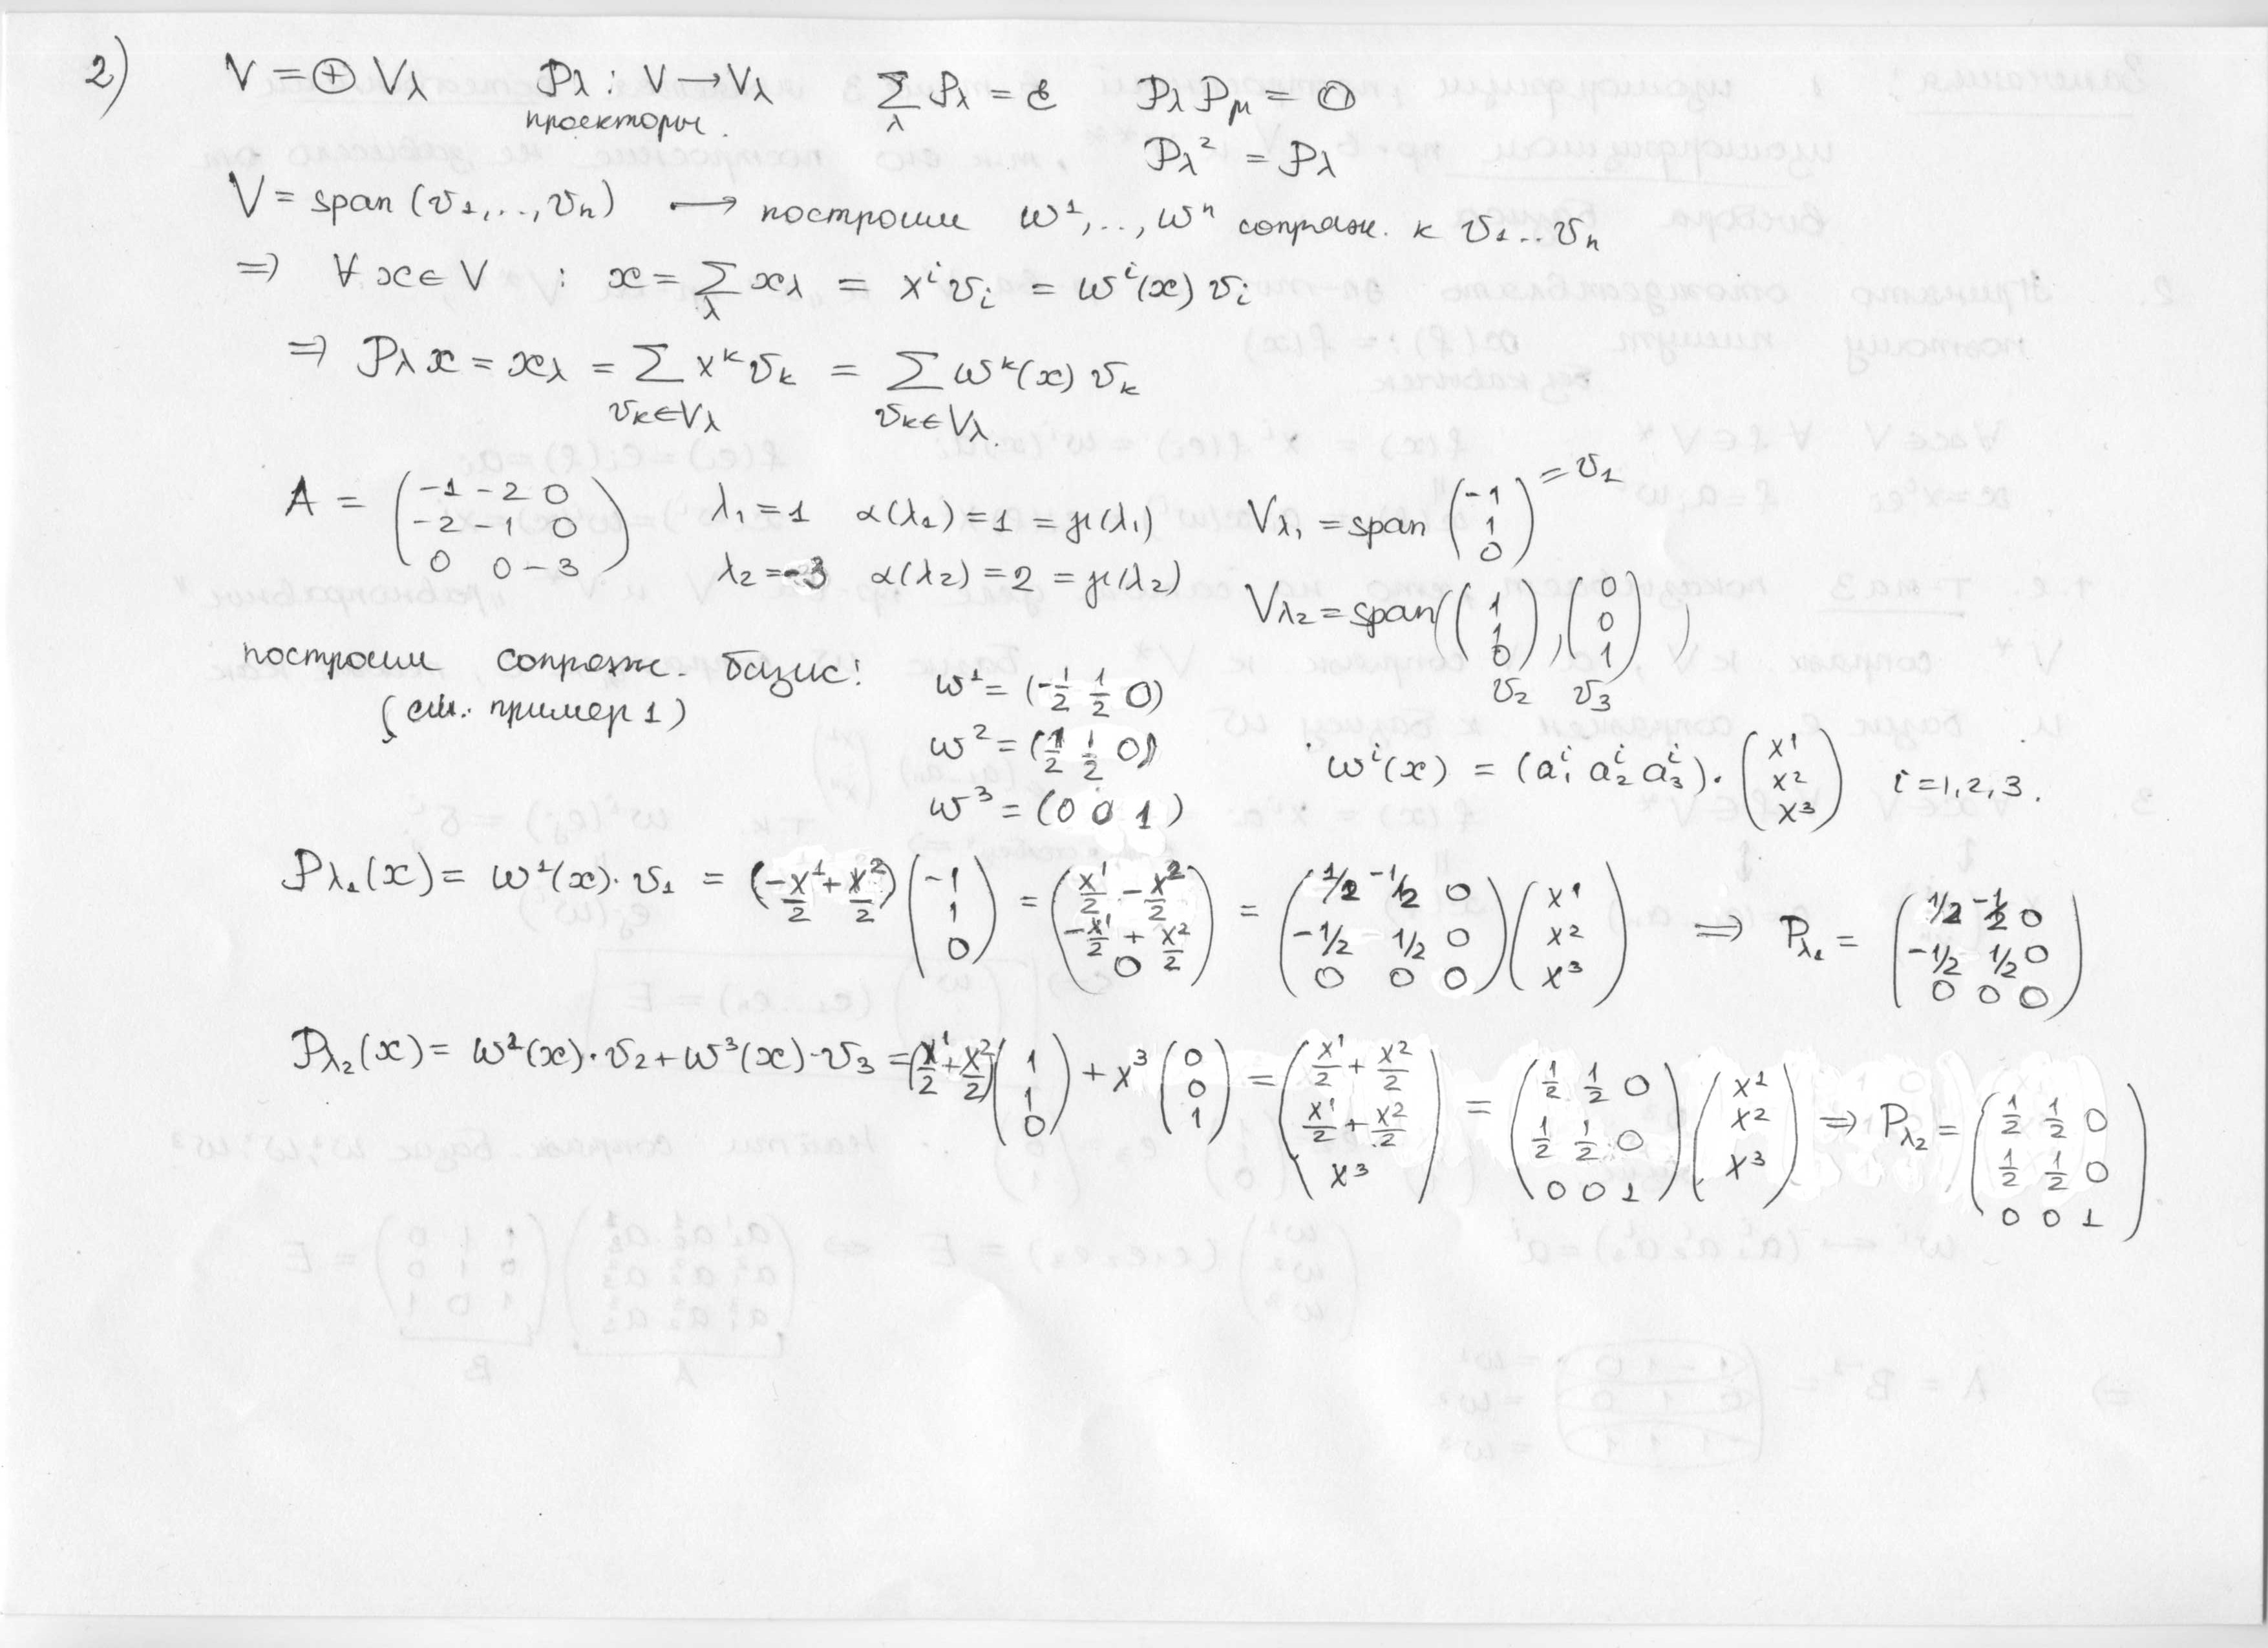
\includegraphics[height=\textheight * 10 / 21, width=\textwidth]{8_1-6}	
		\newline
	\subsection{Два определения тензора. Многомерная матрица. Линейной пространство тензоров.}
	 		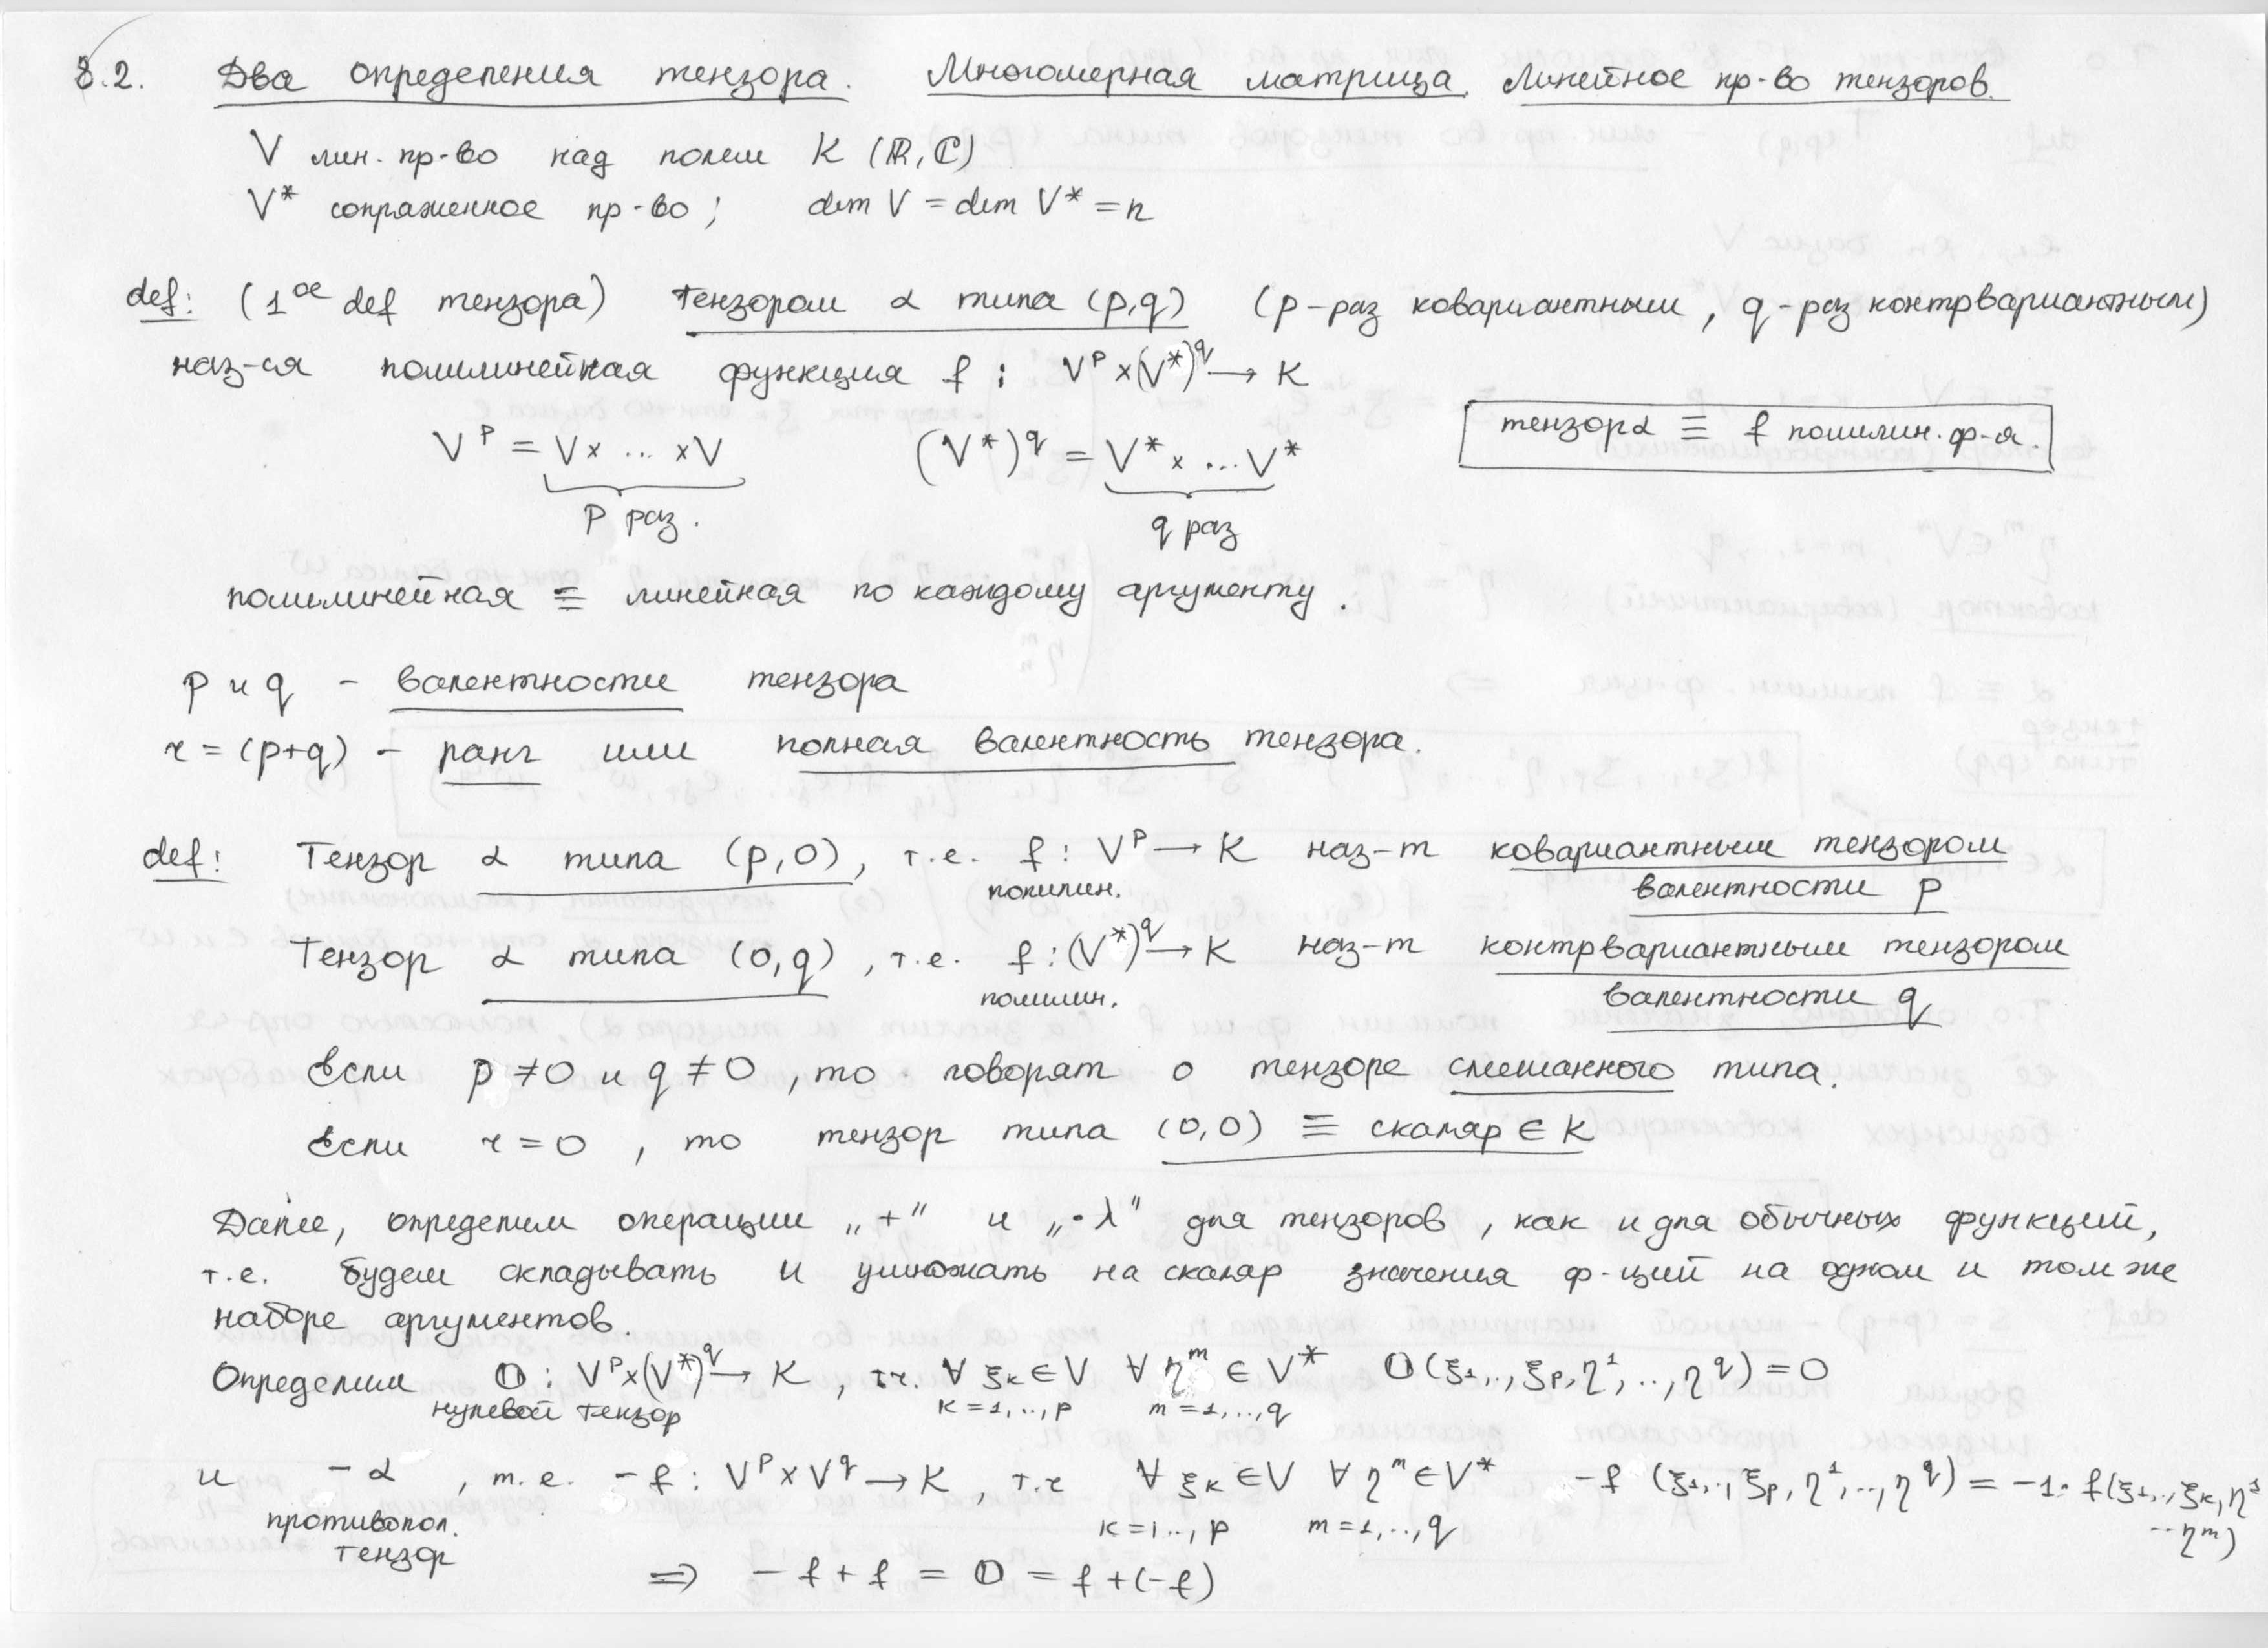
\includegraphics[height=\textheight * 10 / 21, width=\textwidth]{8_2-1}	
		\newline
		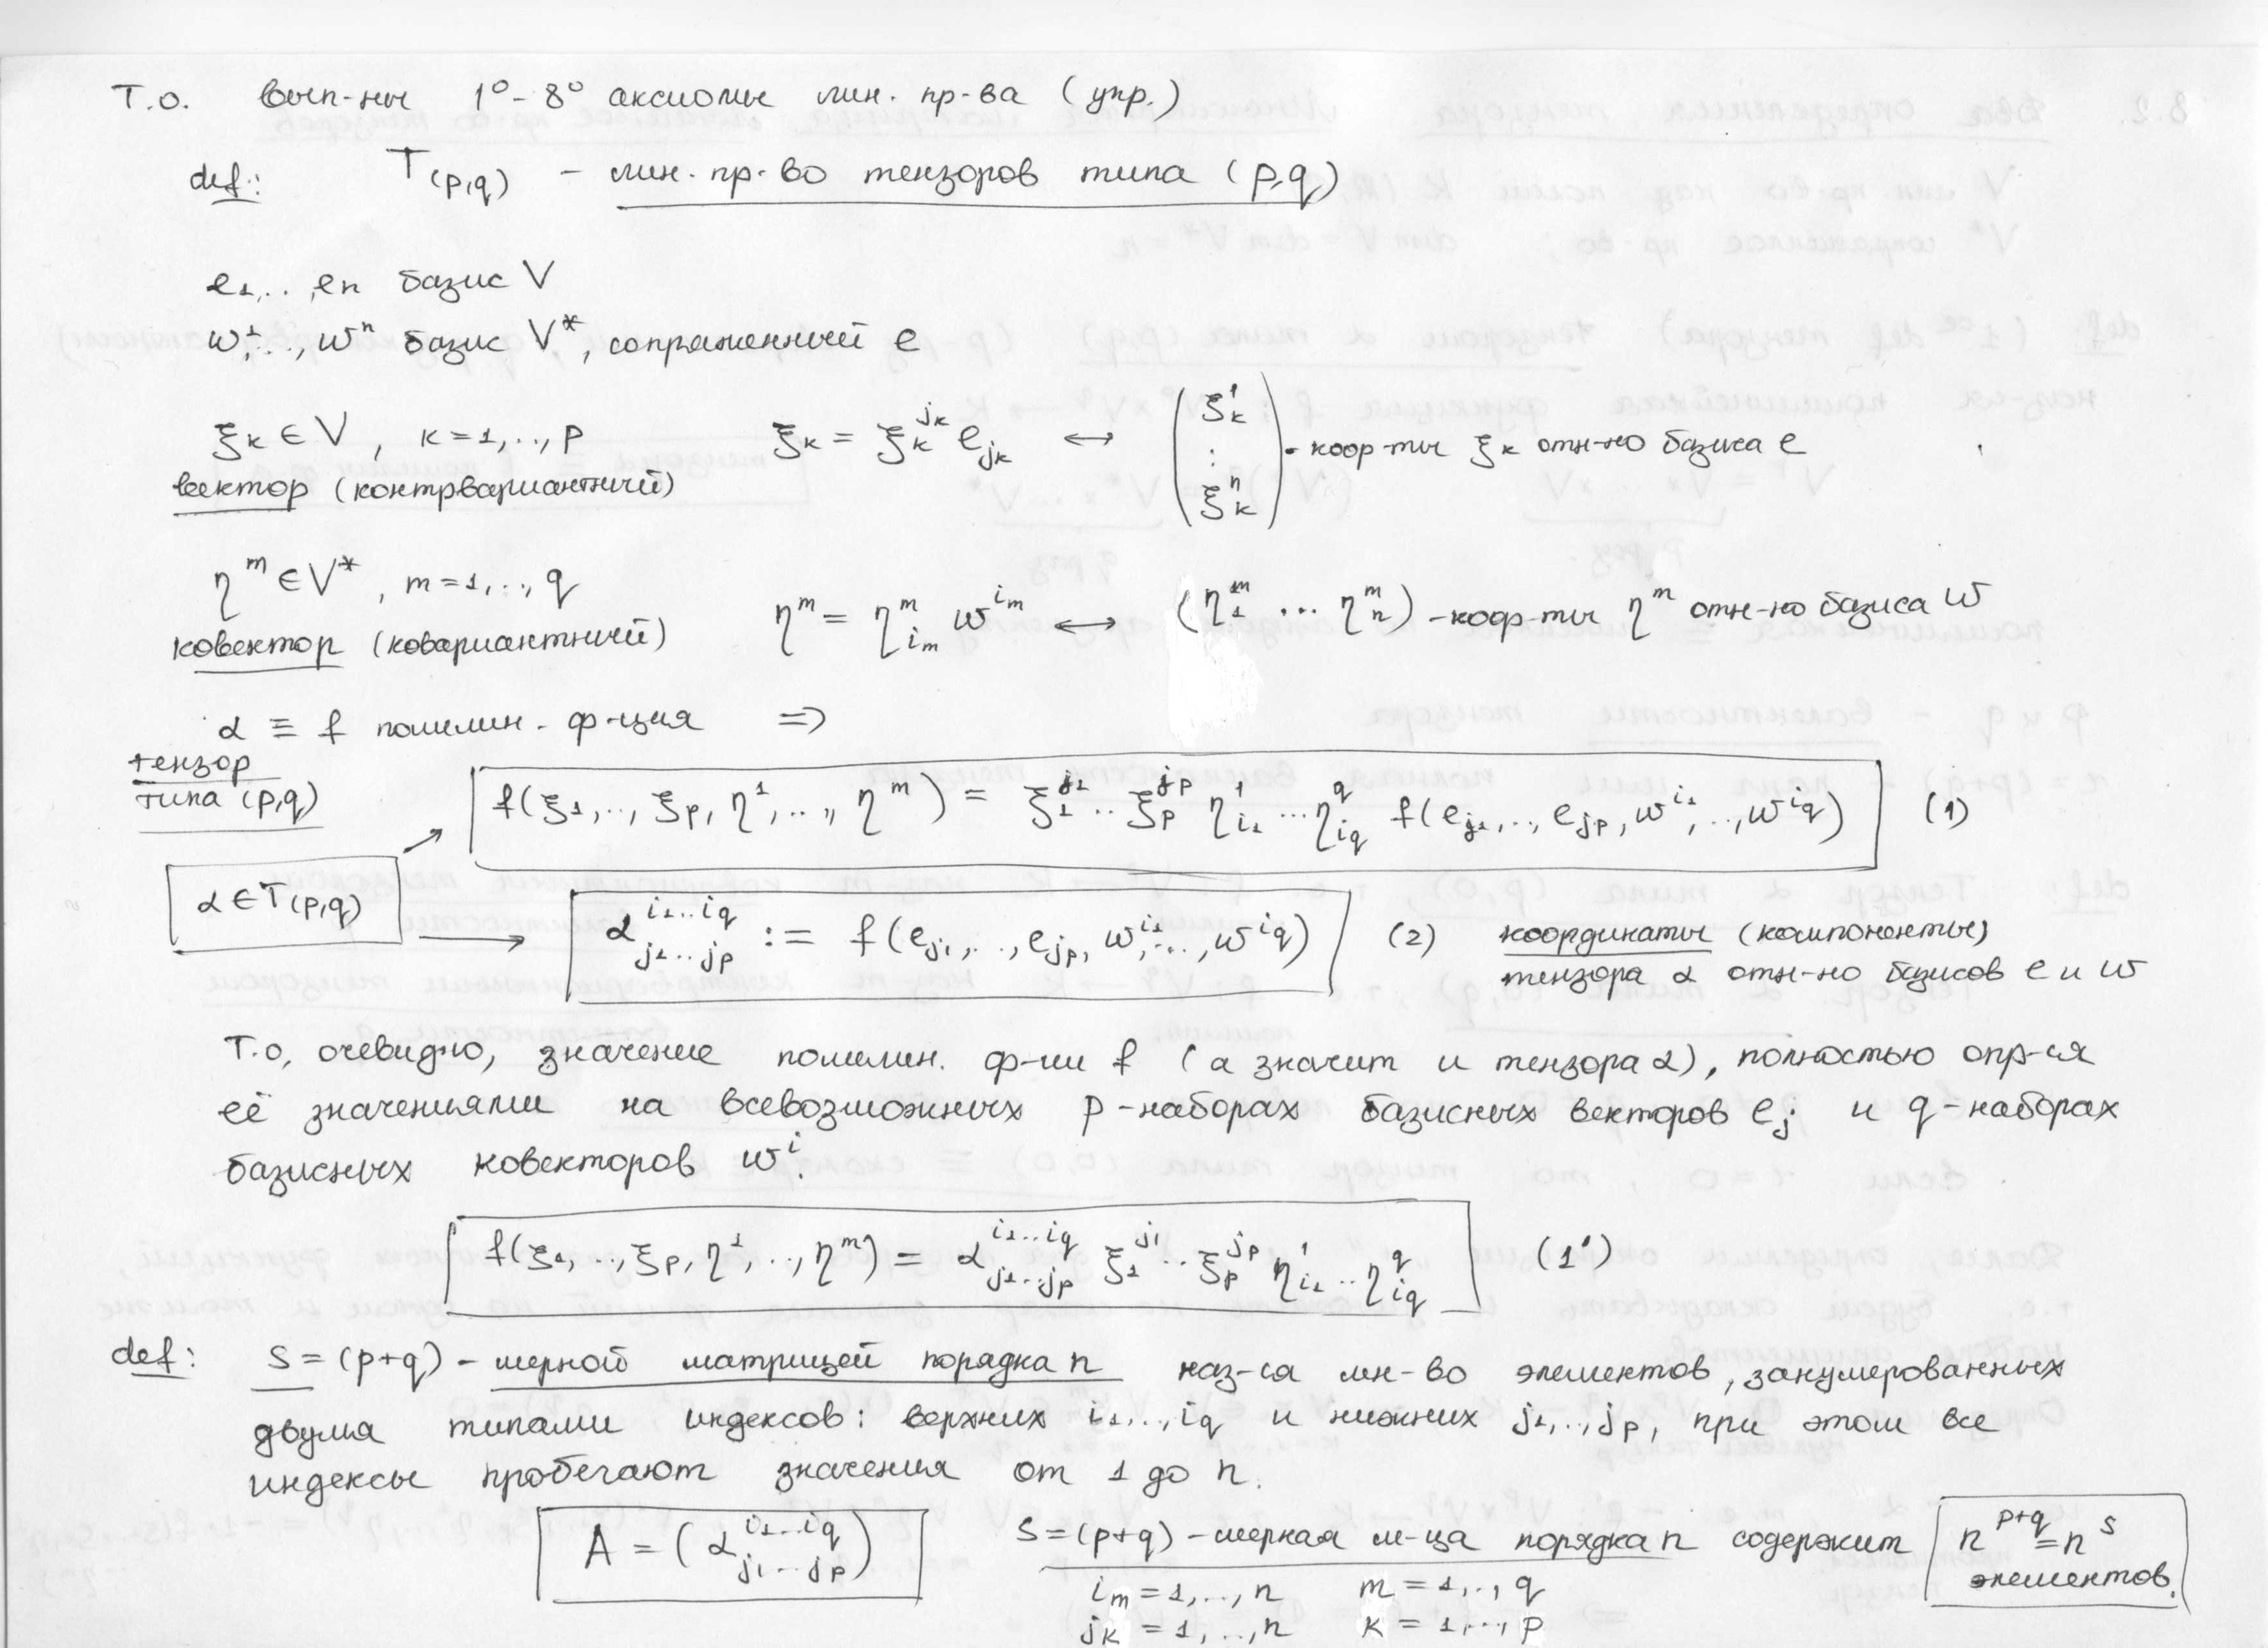
\includegraphics[height=\textheight * 10 / 21, width=\textwidth]{8_2-2}	
		\newline
		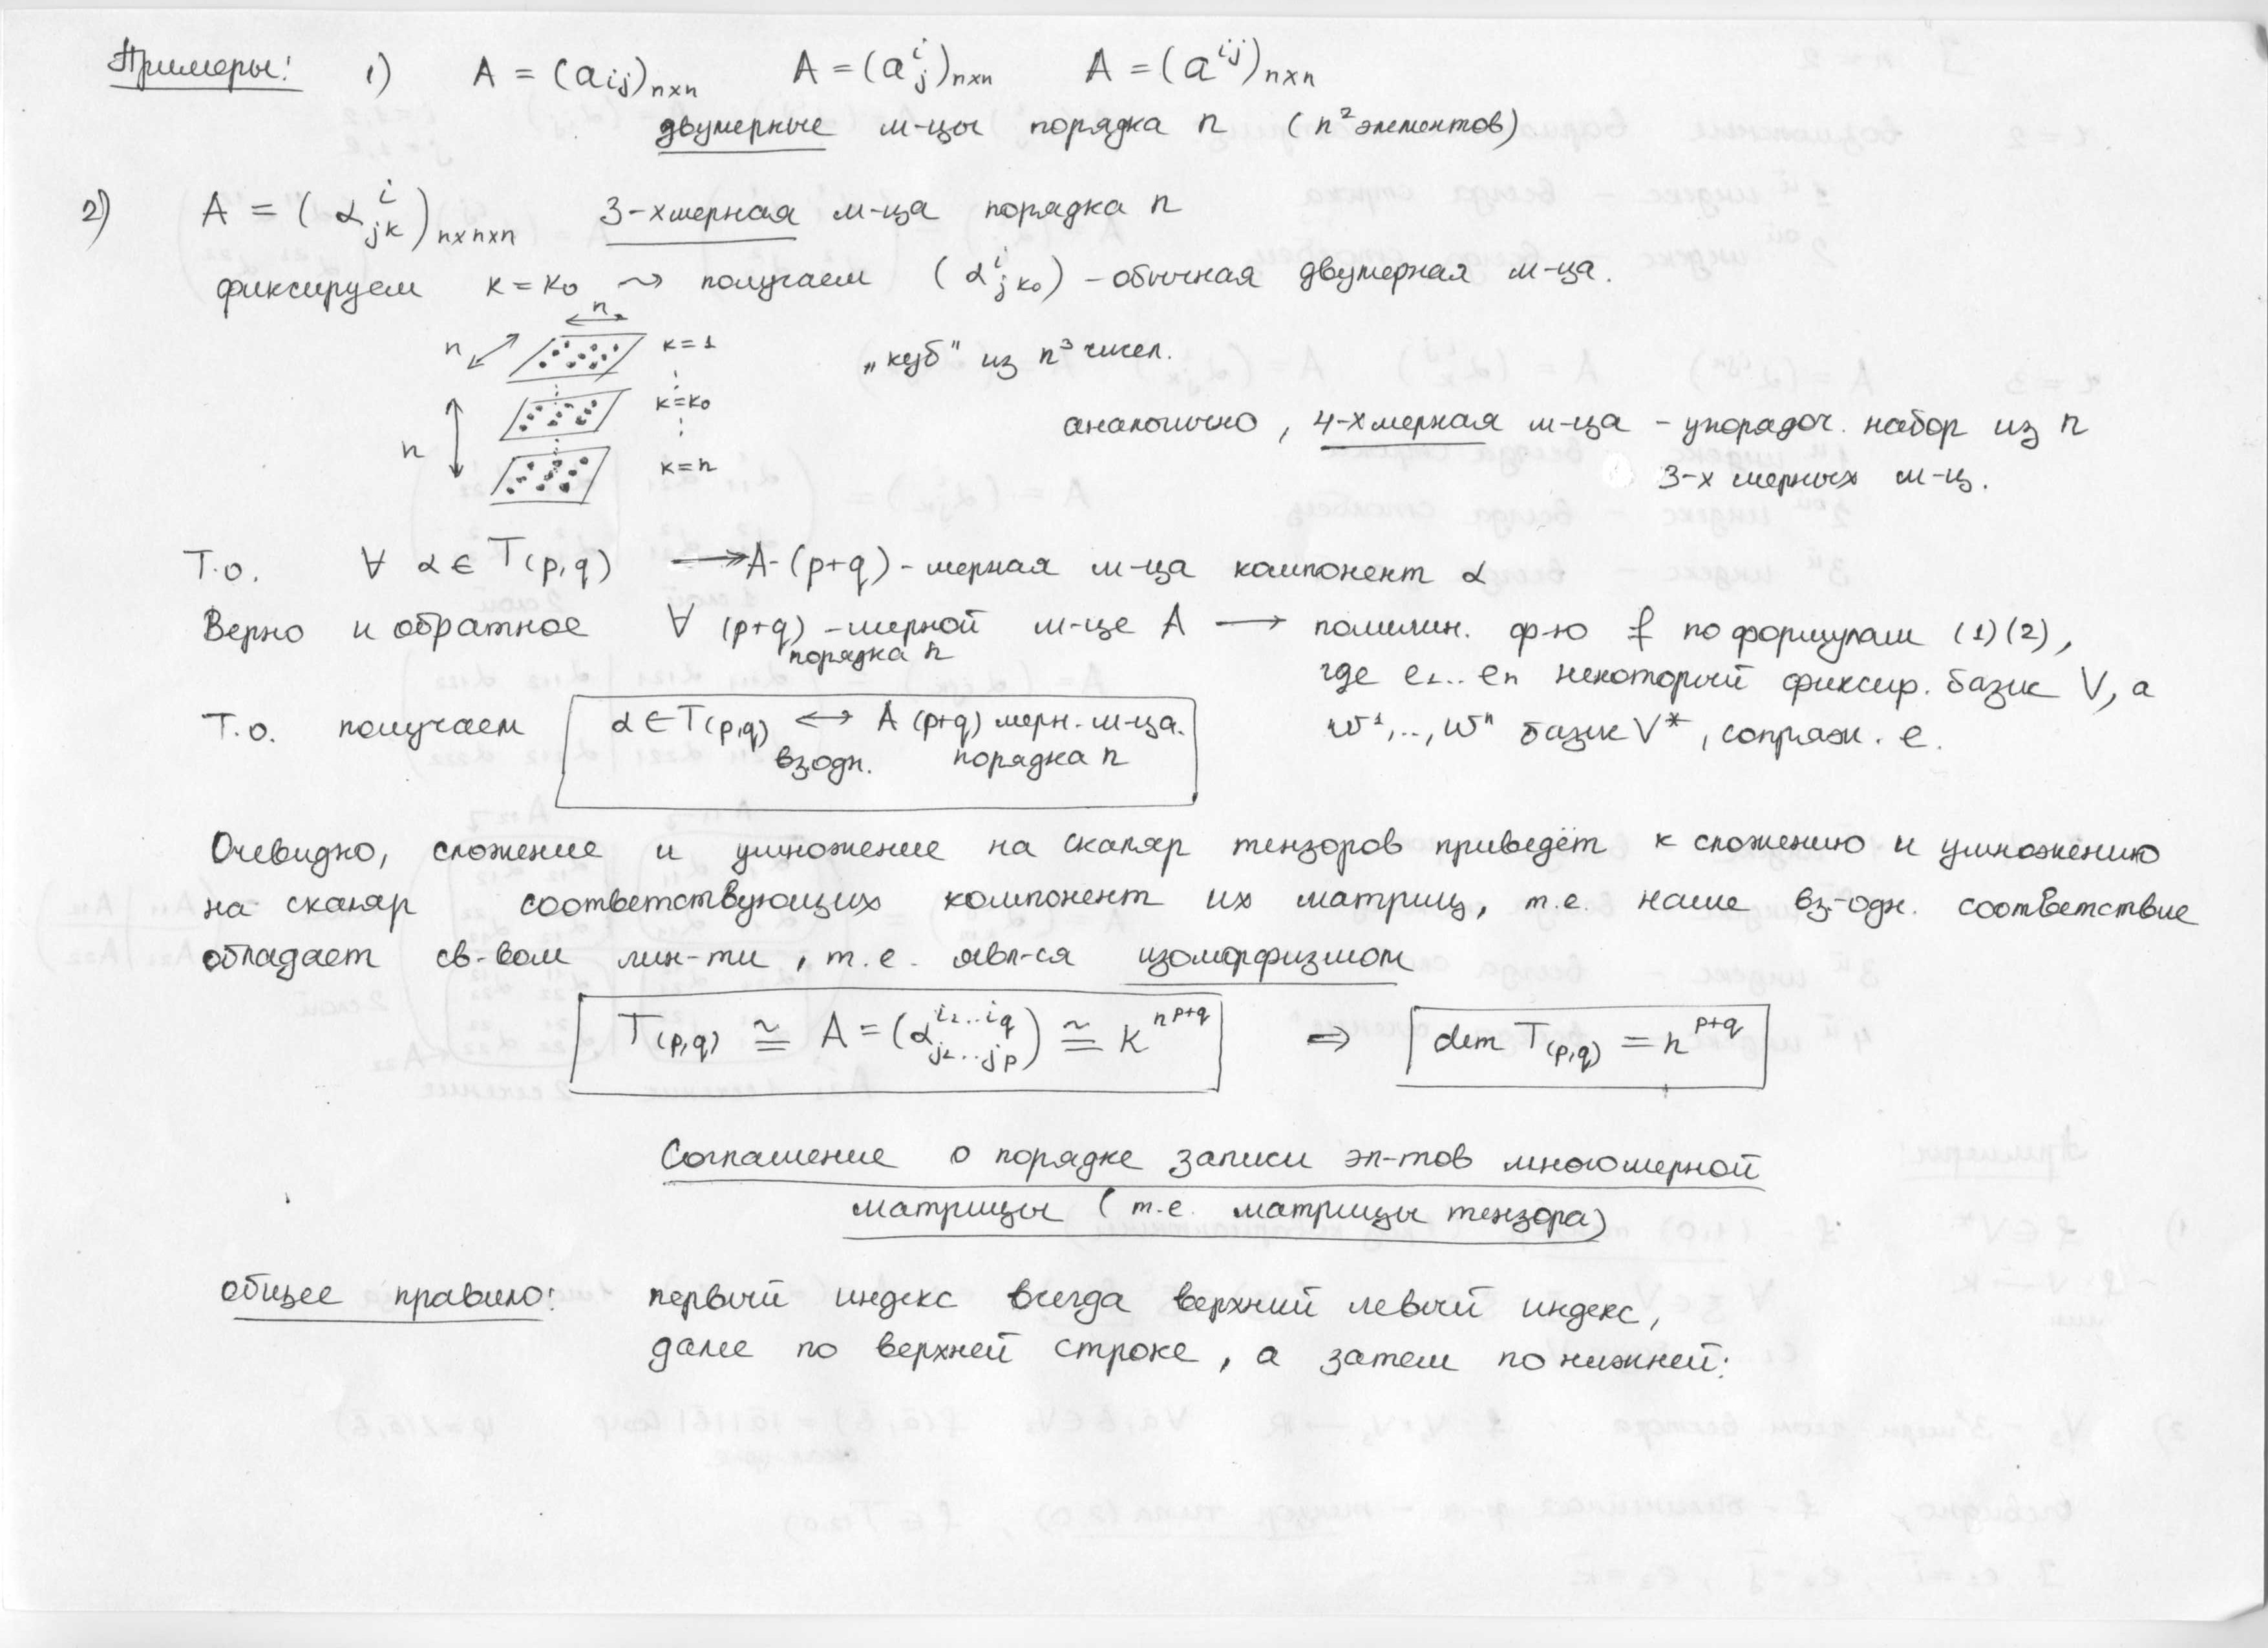
\includegraphics[height=\textheight * 10 / 21, width=\textwidth]{8_2-3}	
		\newline
		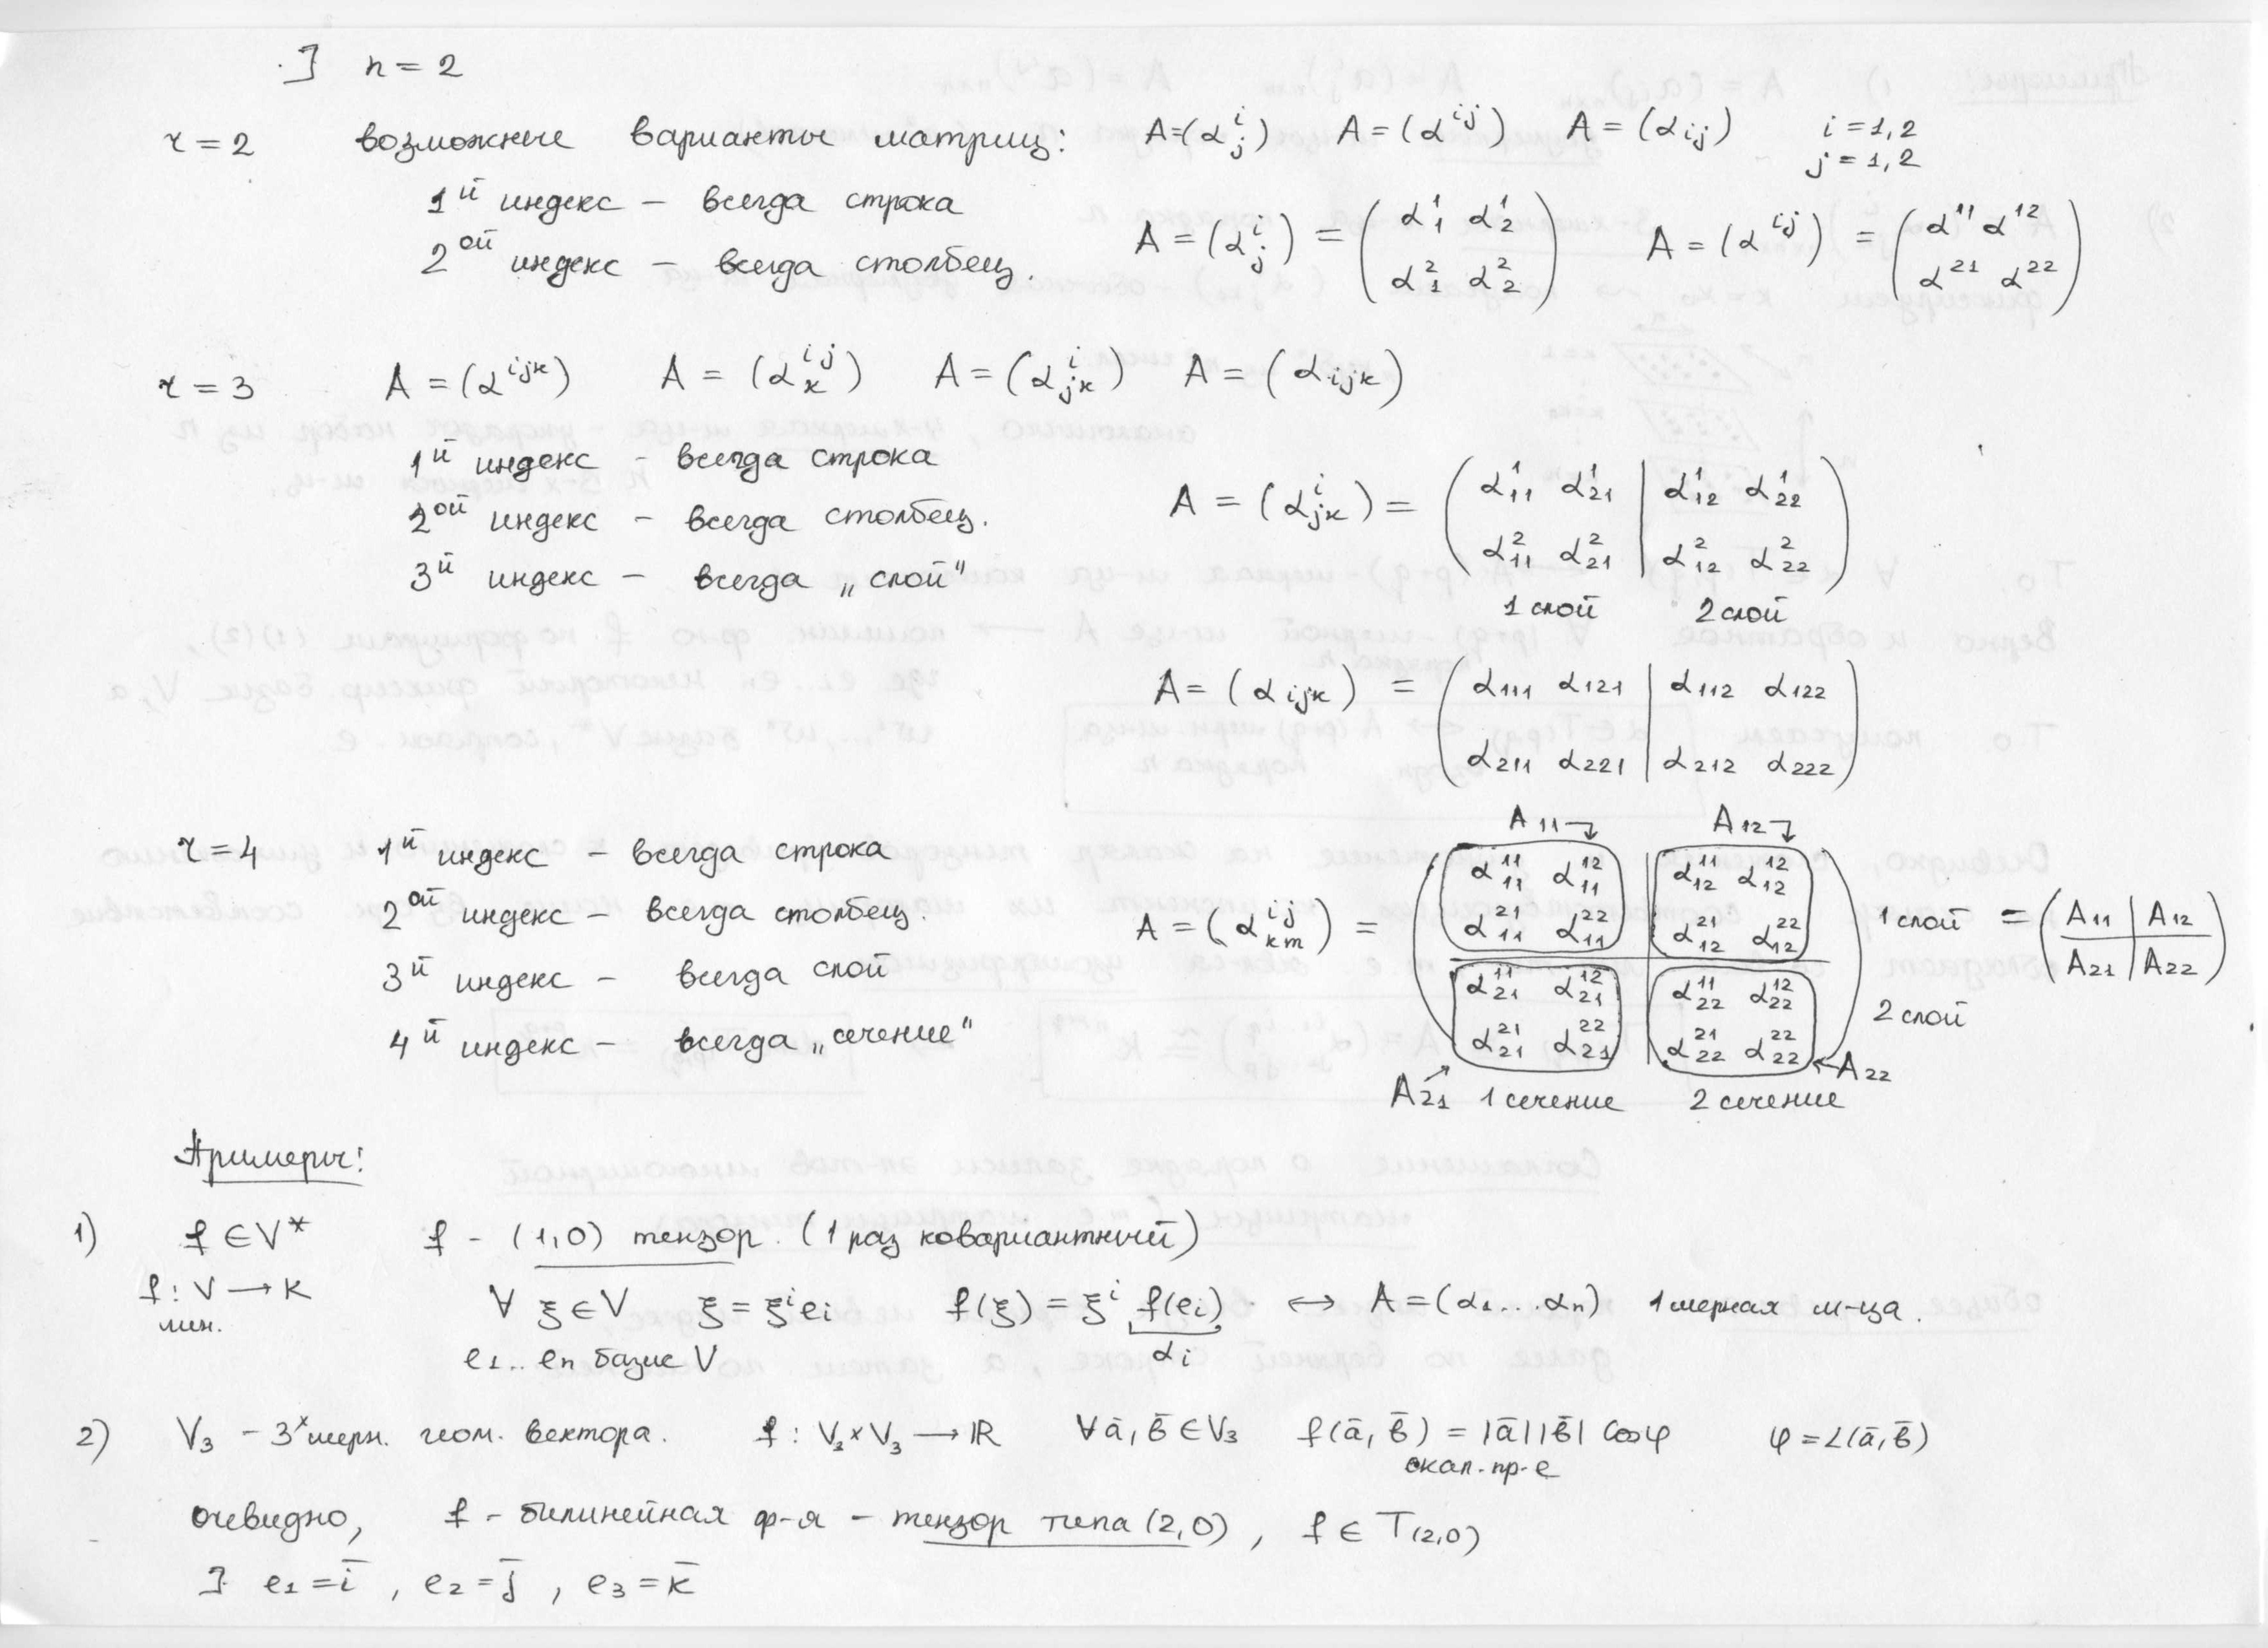
\includegraphics[height=\textheight * 10 / 21, width=\textwidth]{8_2-4}	
		\newline
		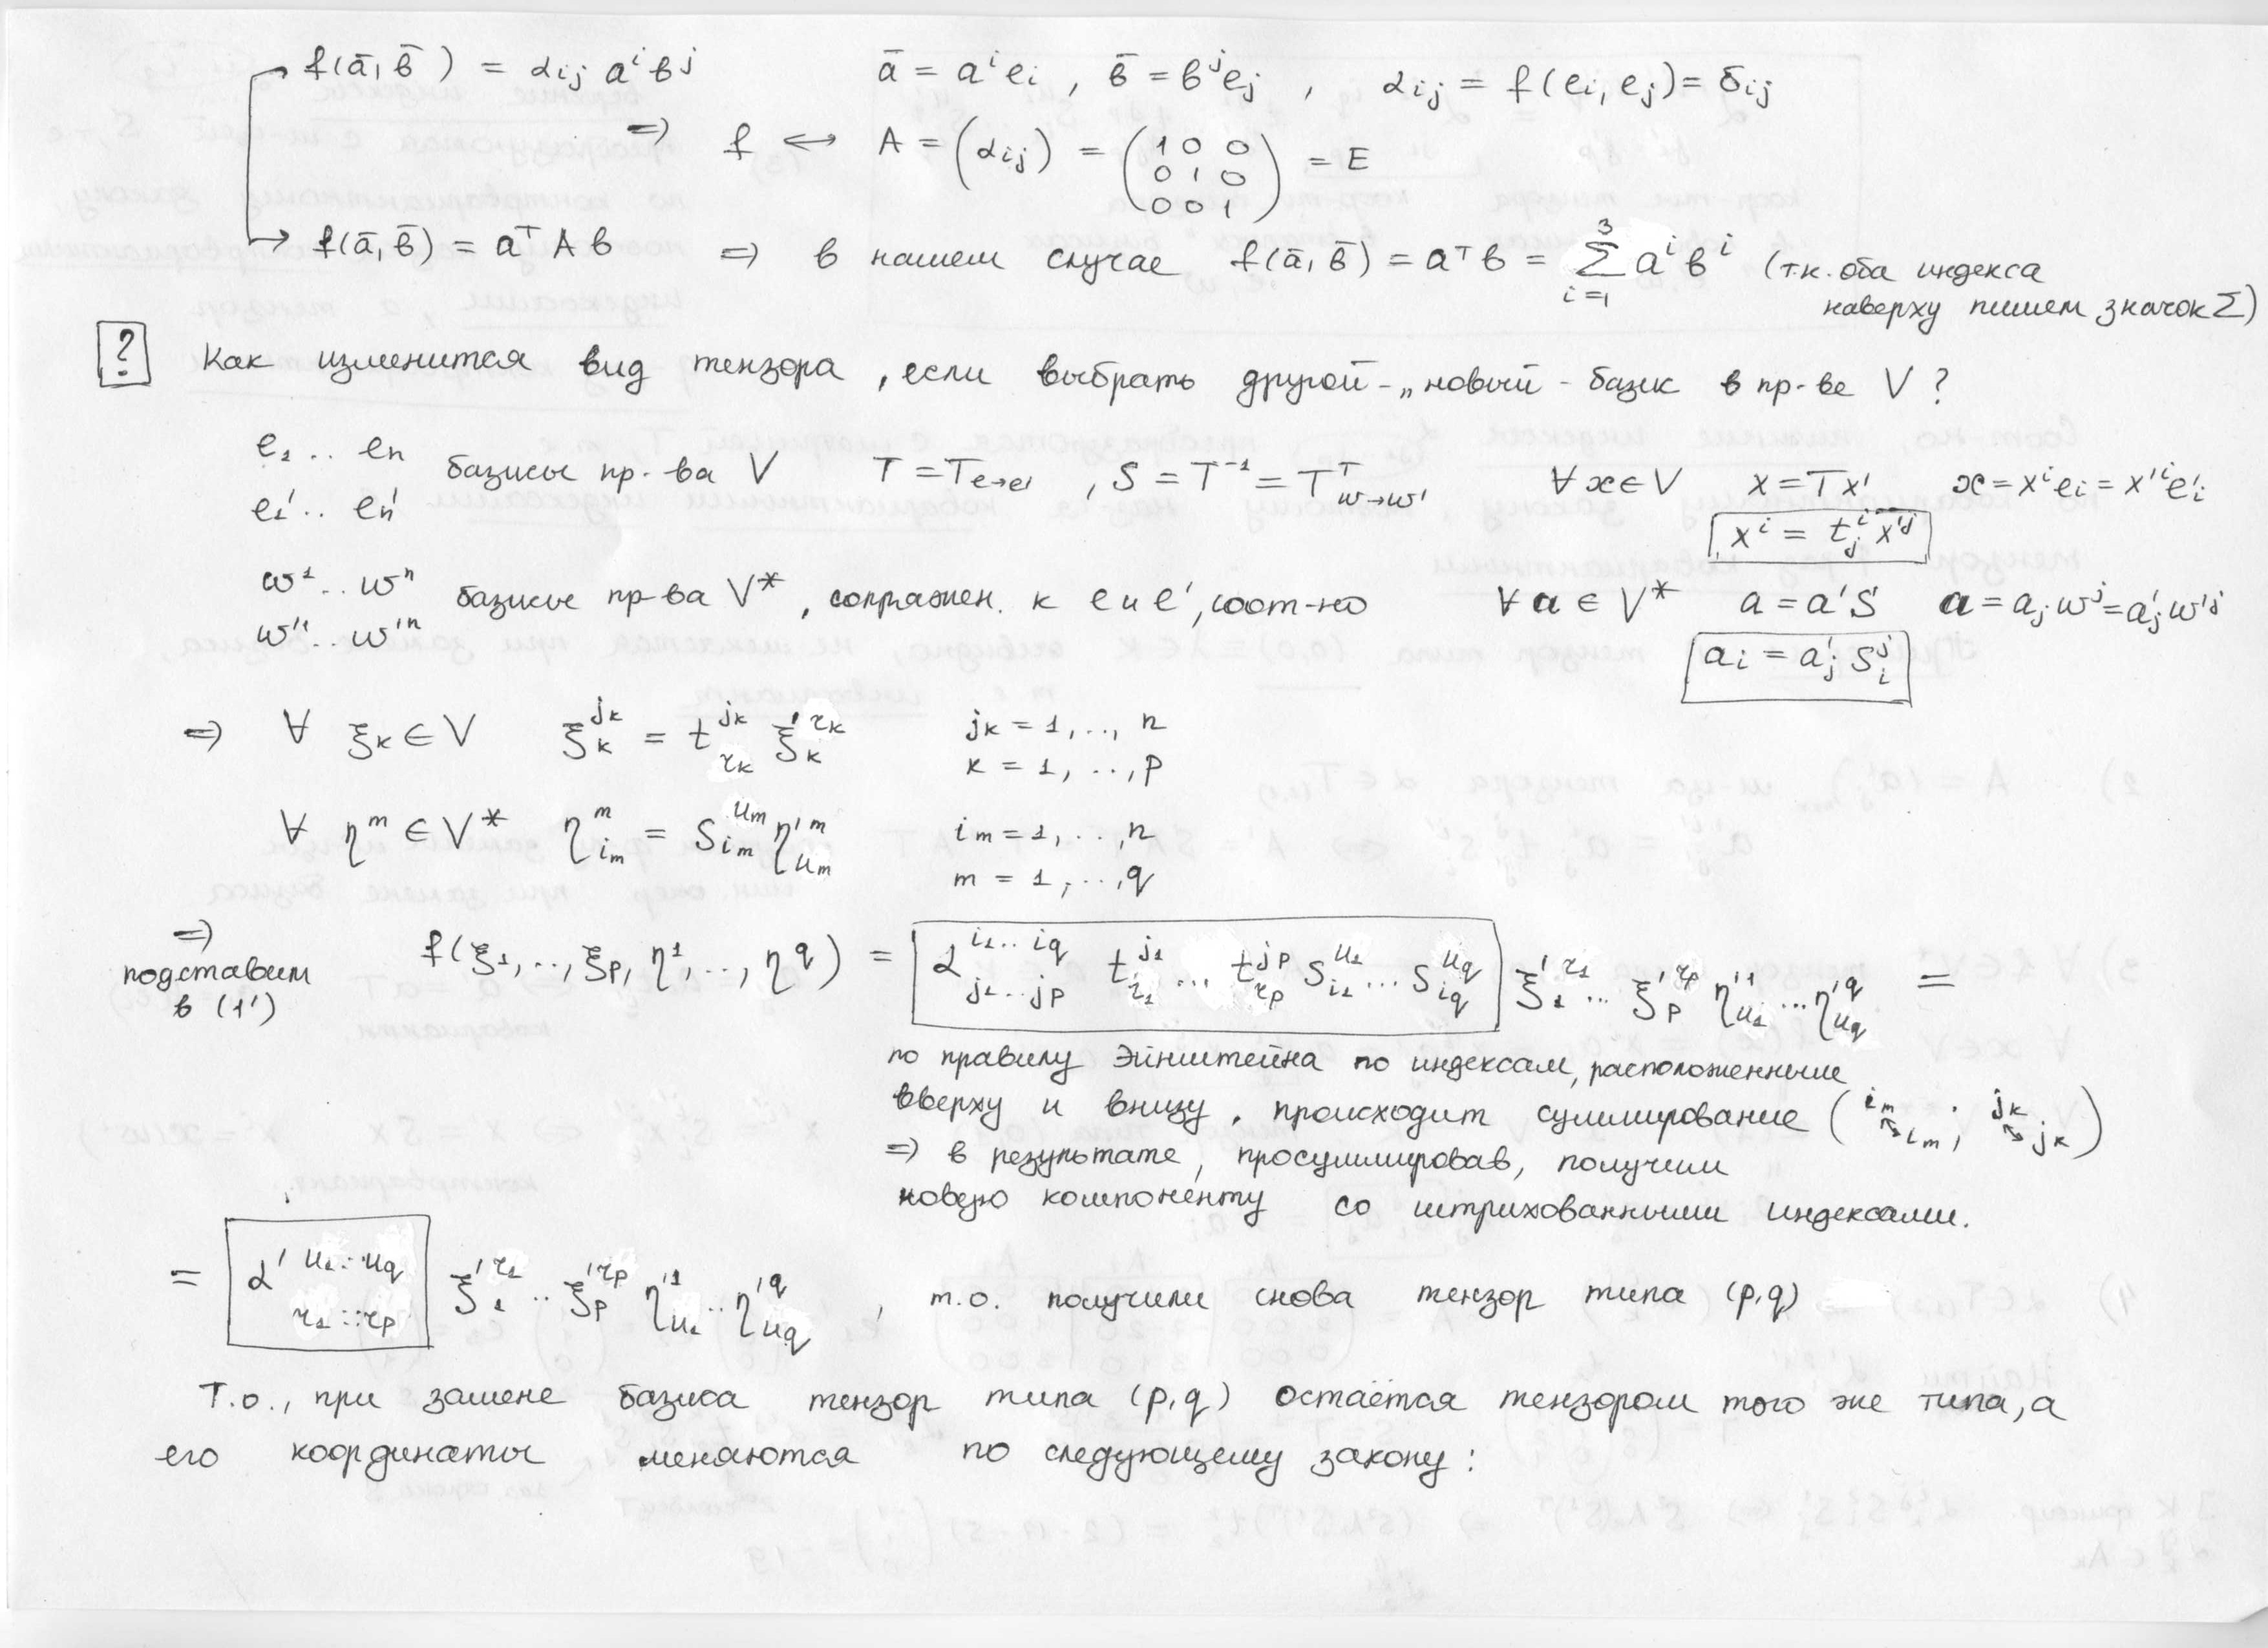
\includegraphics[height=\textheight * 10 / 21, width=\textwidth]{8_2-5}	
		\newline
		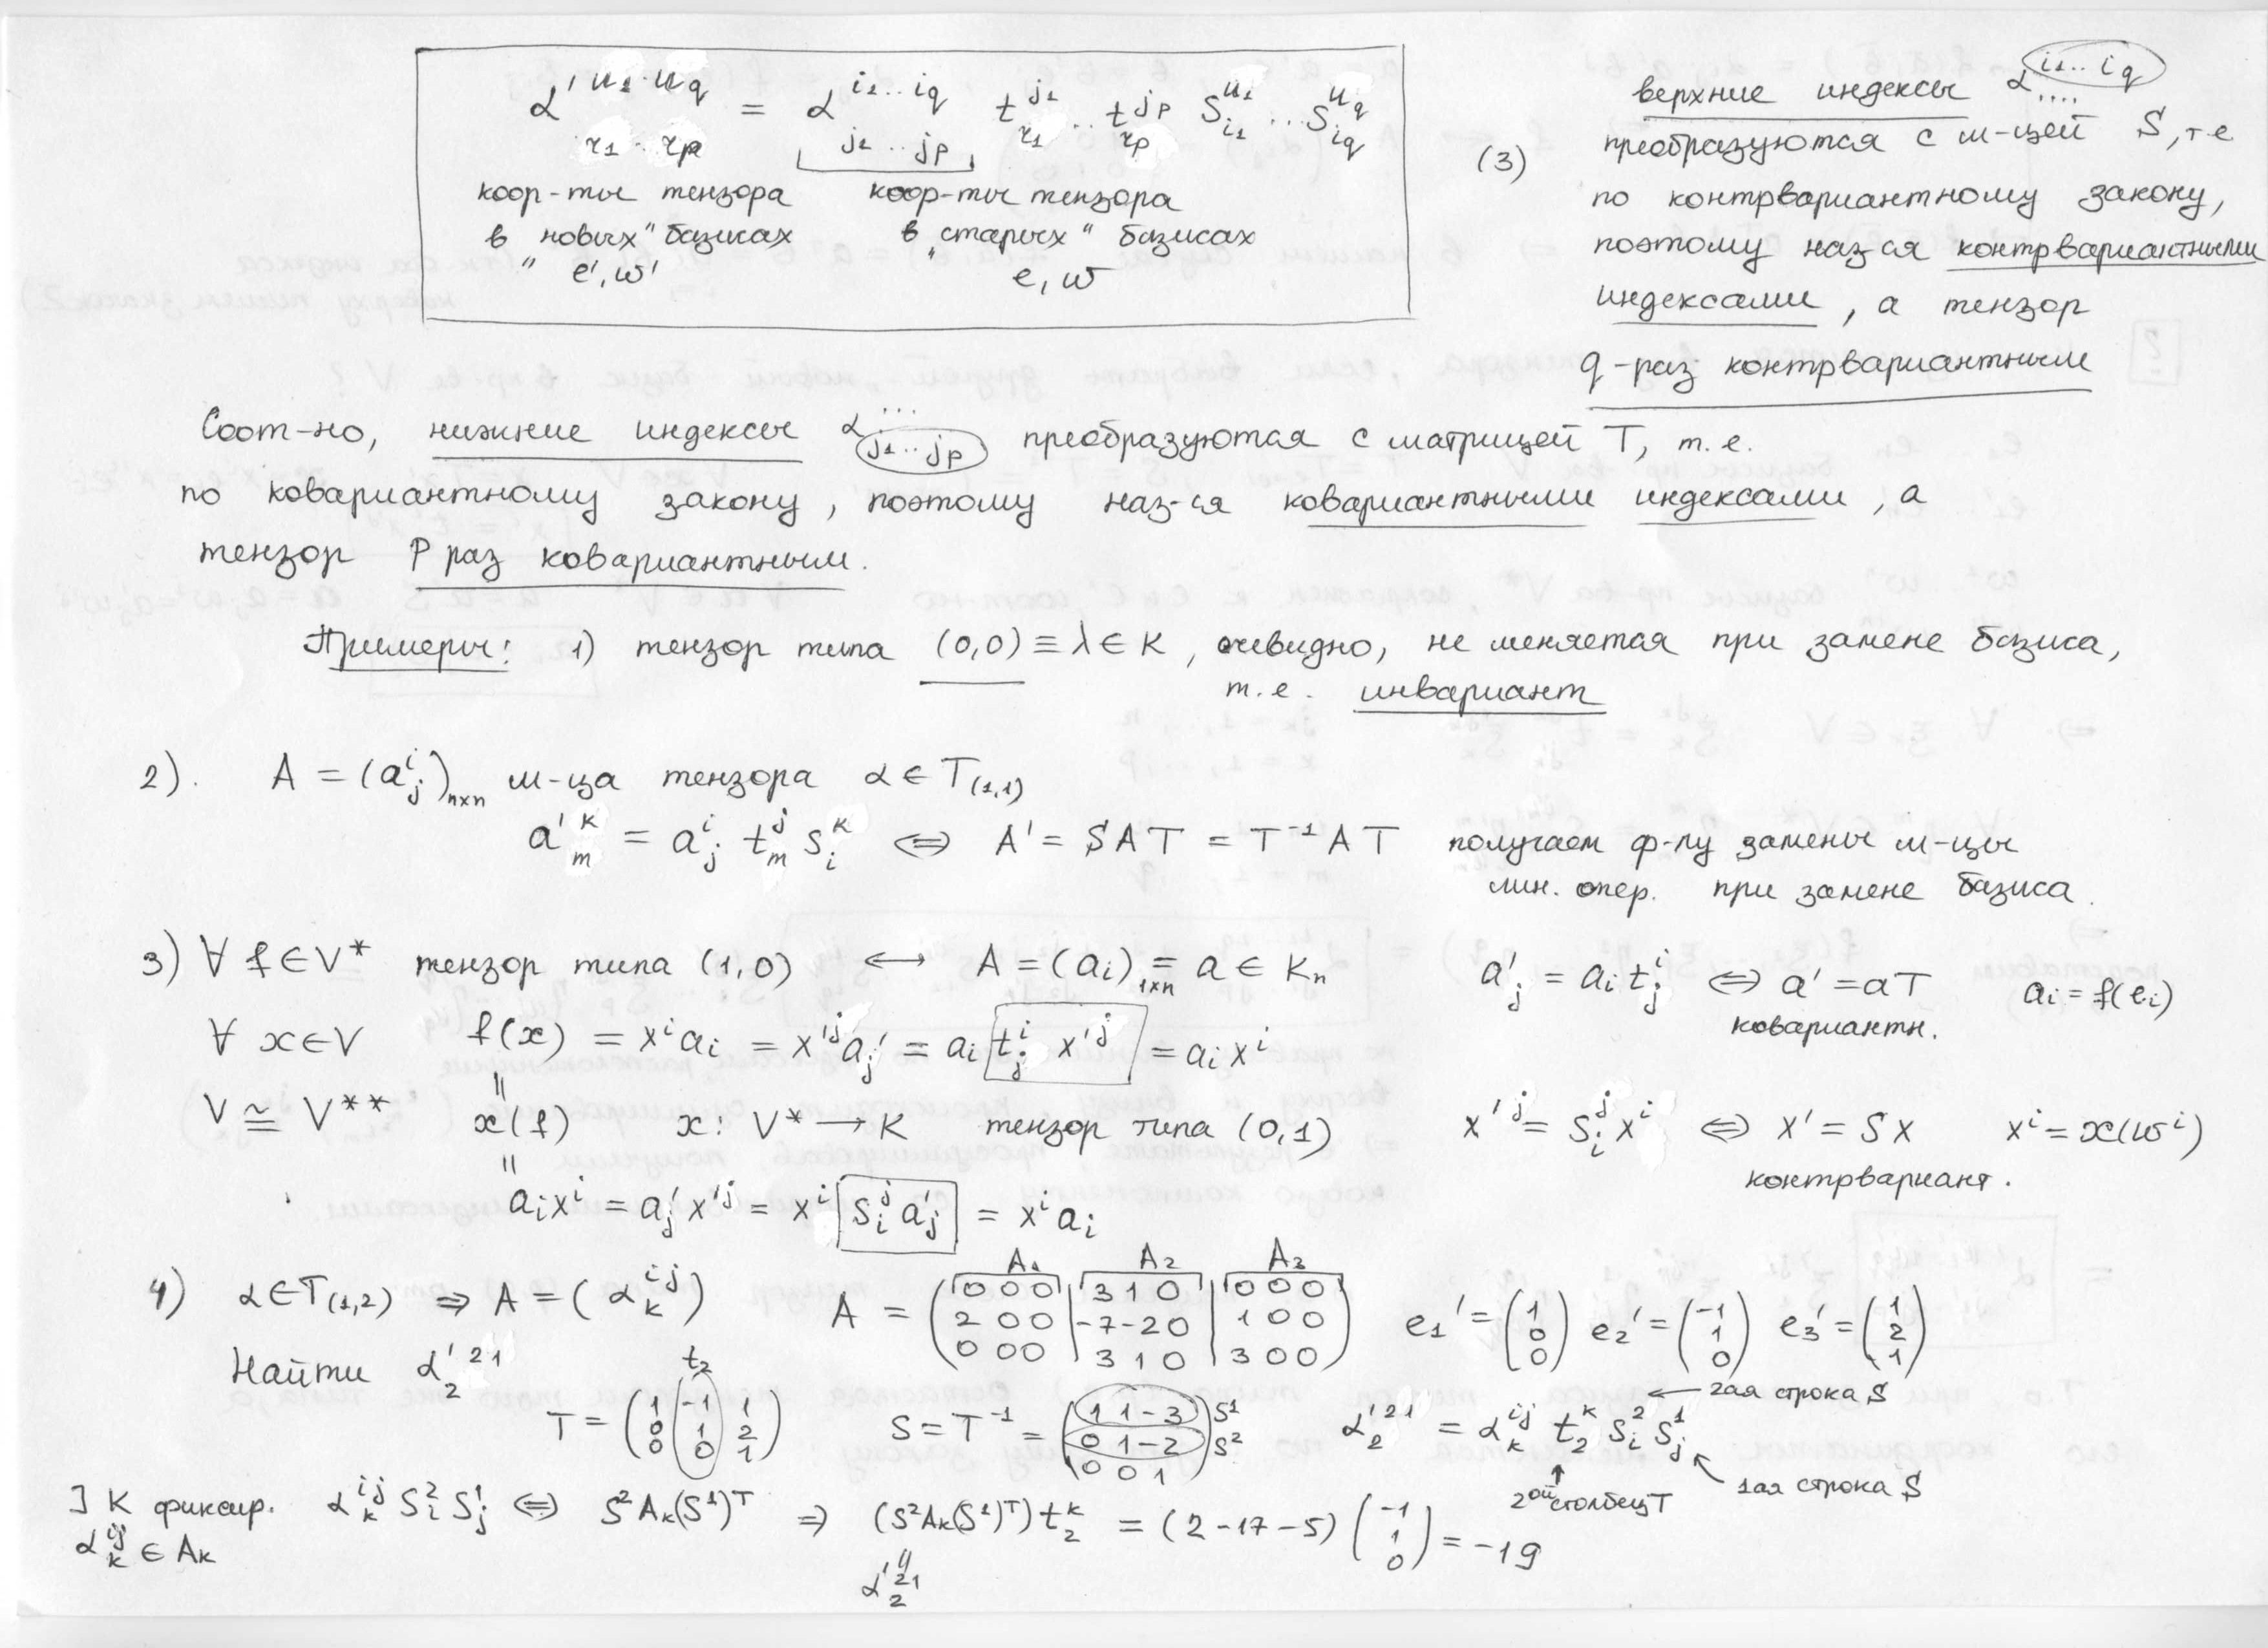
\includegraphics[height=\textheight * 10 / 21, width=\textwidth]{8_2-6}	
		\newline
		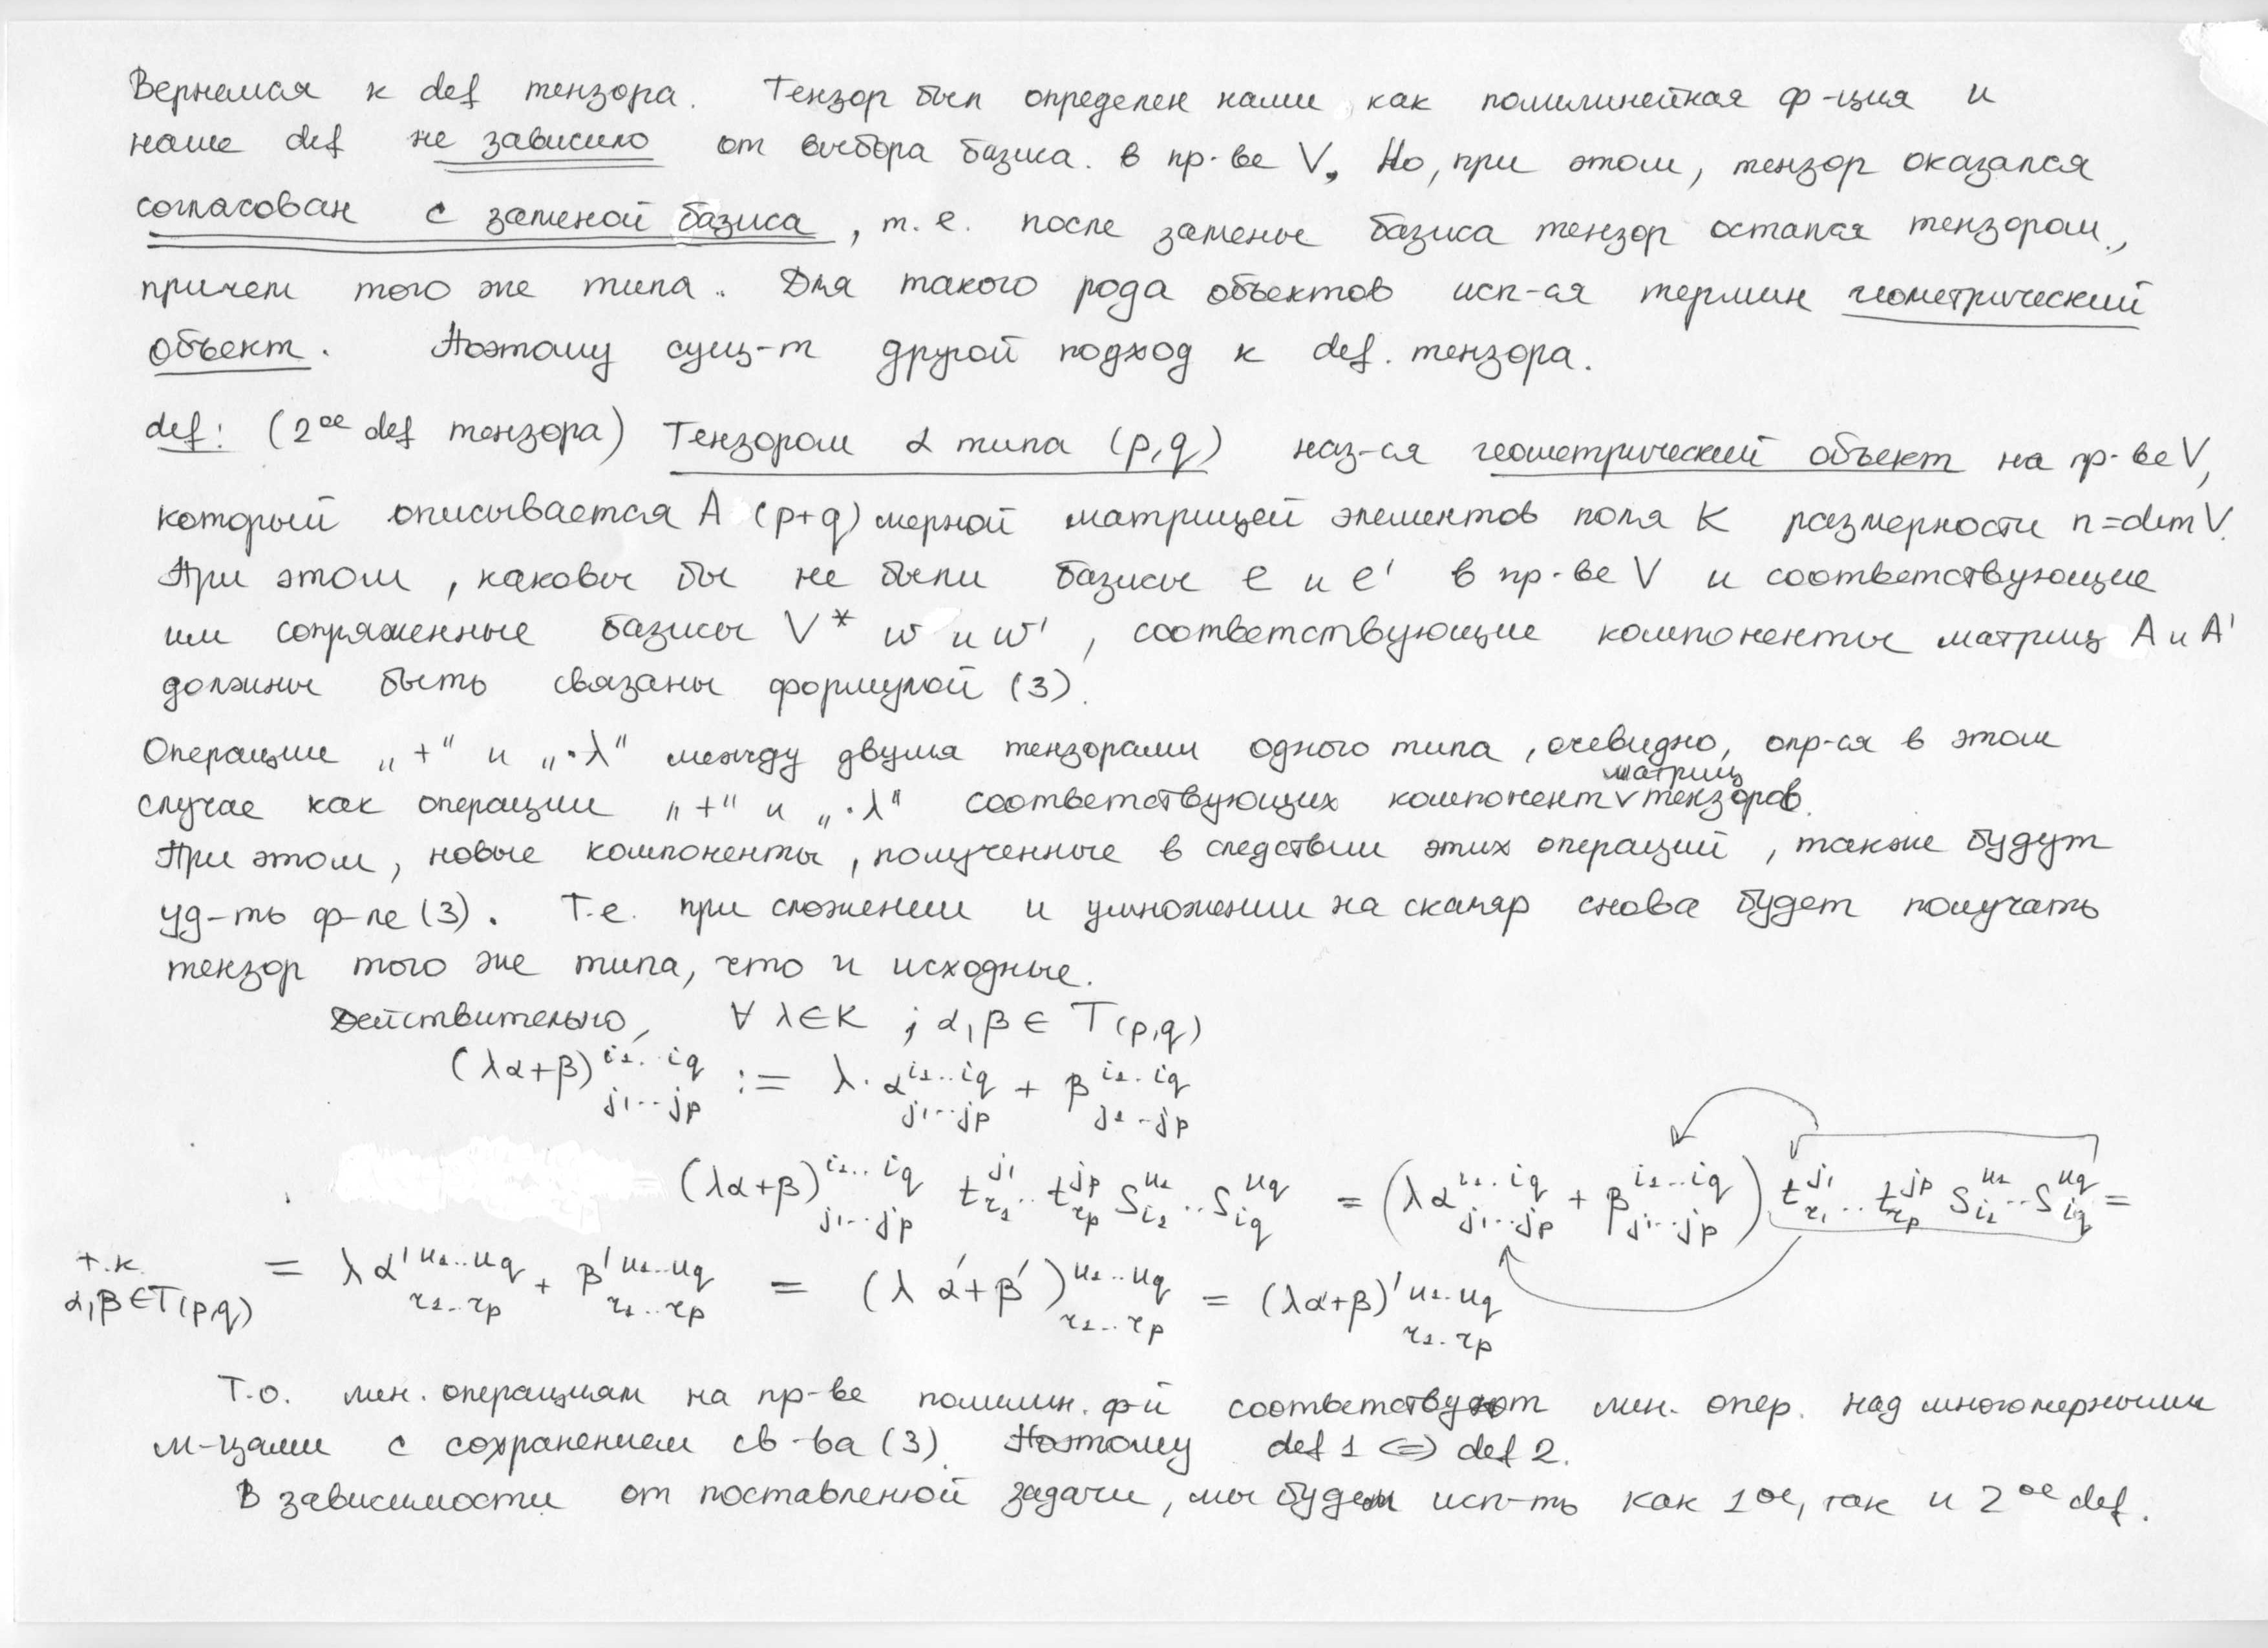
\includegraphics[height=\textheight * 10 / 21, width=\textwidth]{8_2-7}	
		
		
	\subsection{Два определения тензора. Многомерная матрица. Линейной пространство тензоров.}
	 		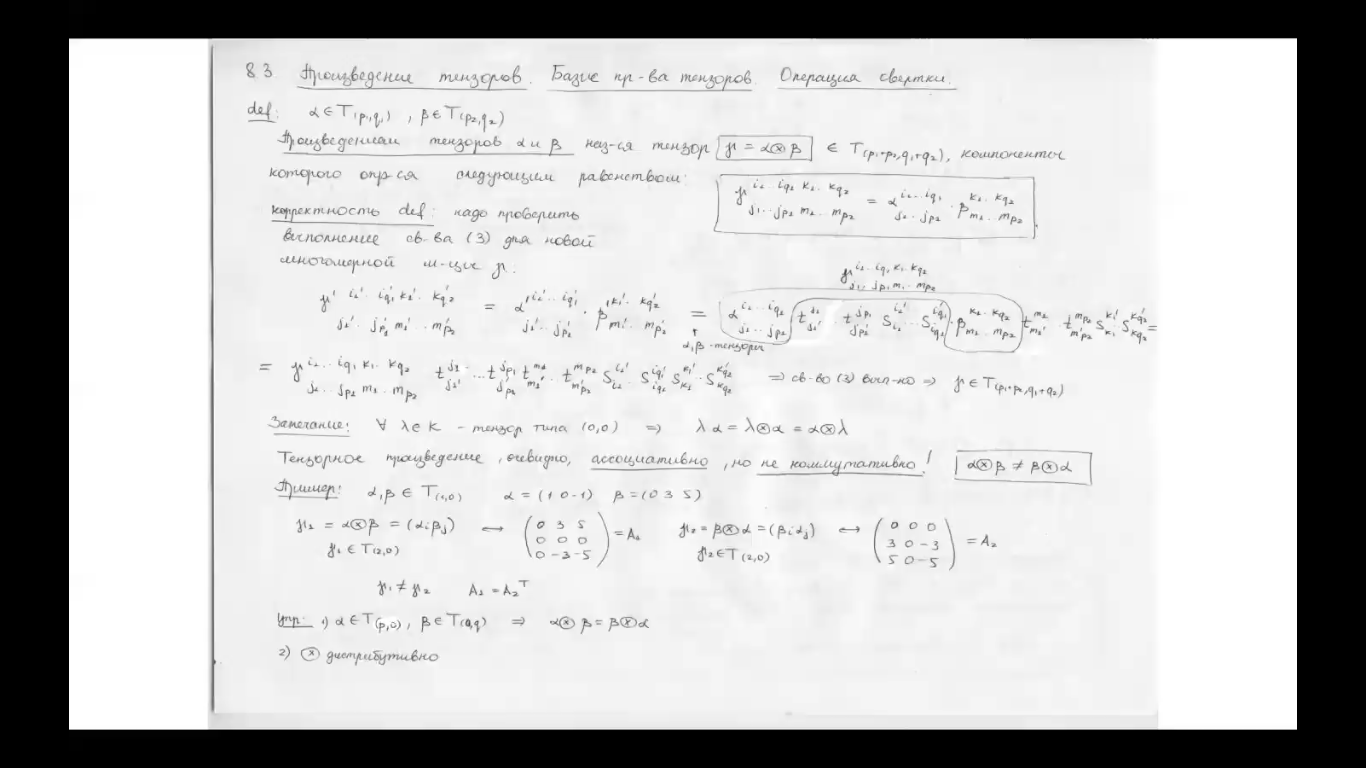
\includegraphics[height=\textheight * 10 / 21, width=\textwidth]{8_3-1}	
		\newline
		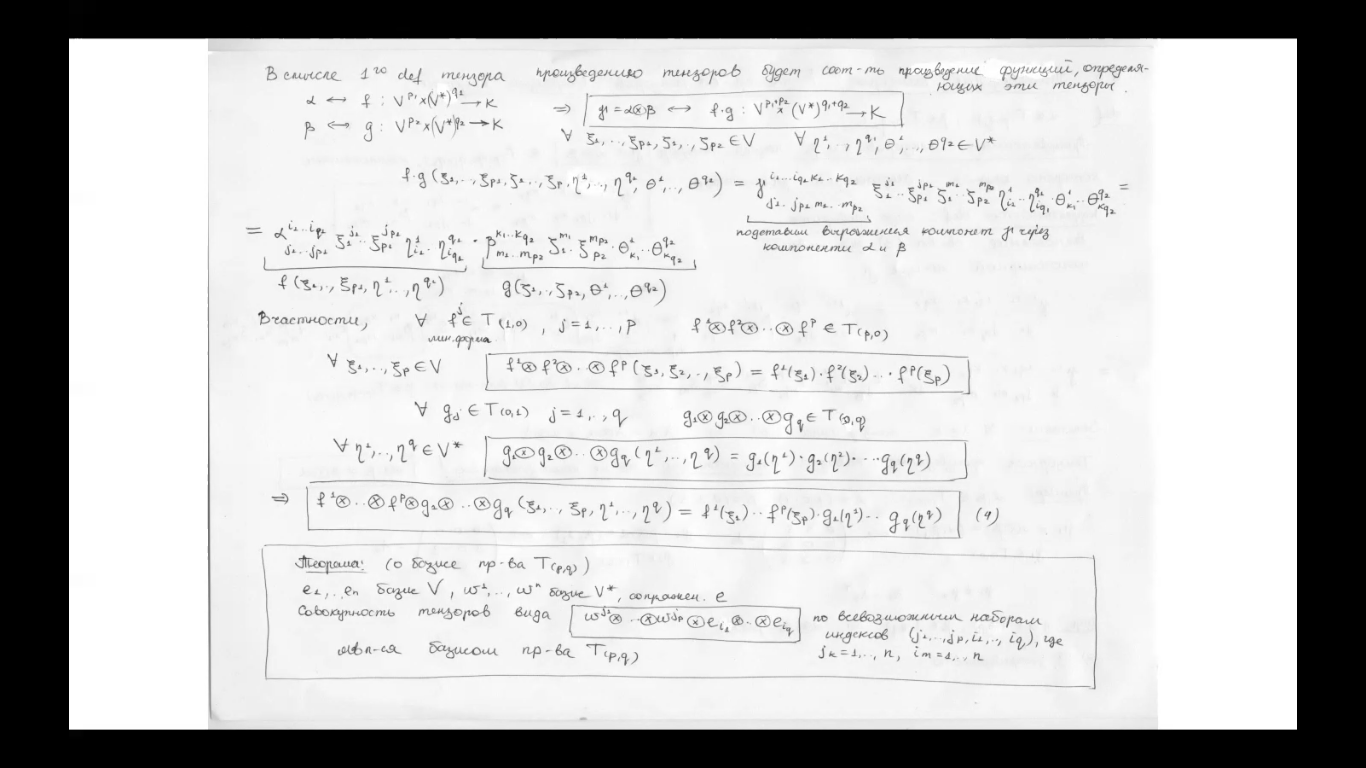
\includegraphics[height=\textheight * 10 / 21, width=\textwidth]{8_3-2}	
		\newline
		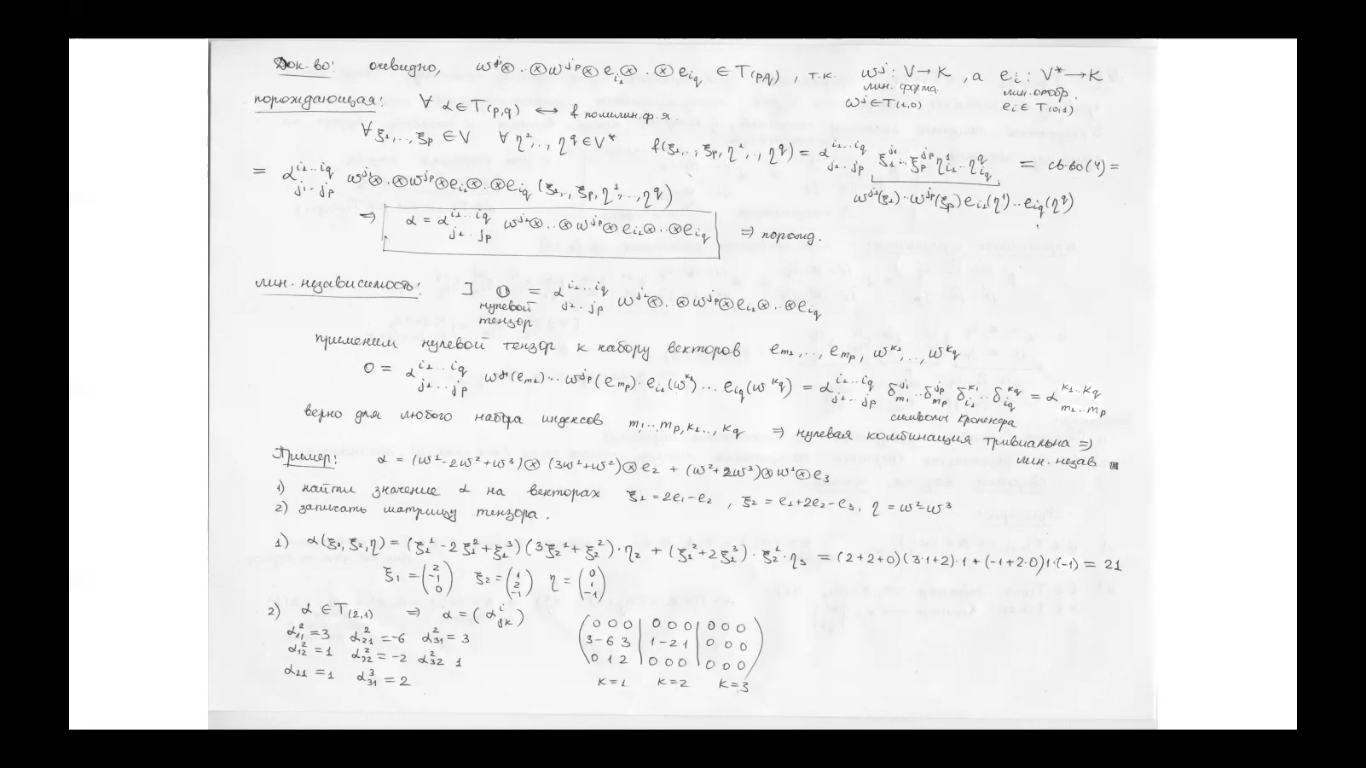
\includegraphics[height=\textheight * 10 / 21, width=\textwidth]{8_3-3}	
		\newline
		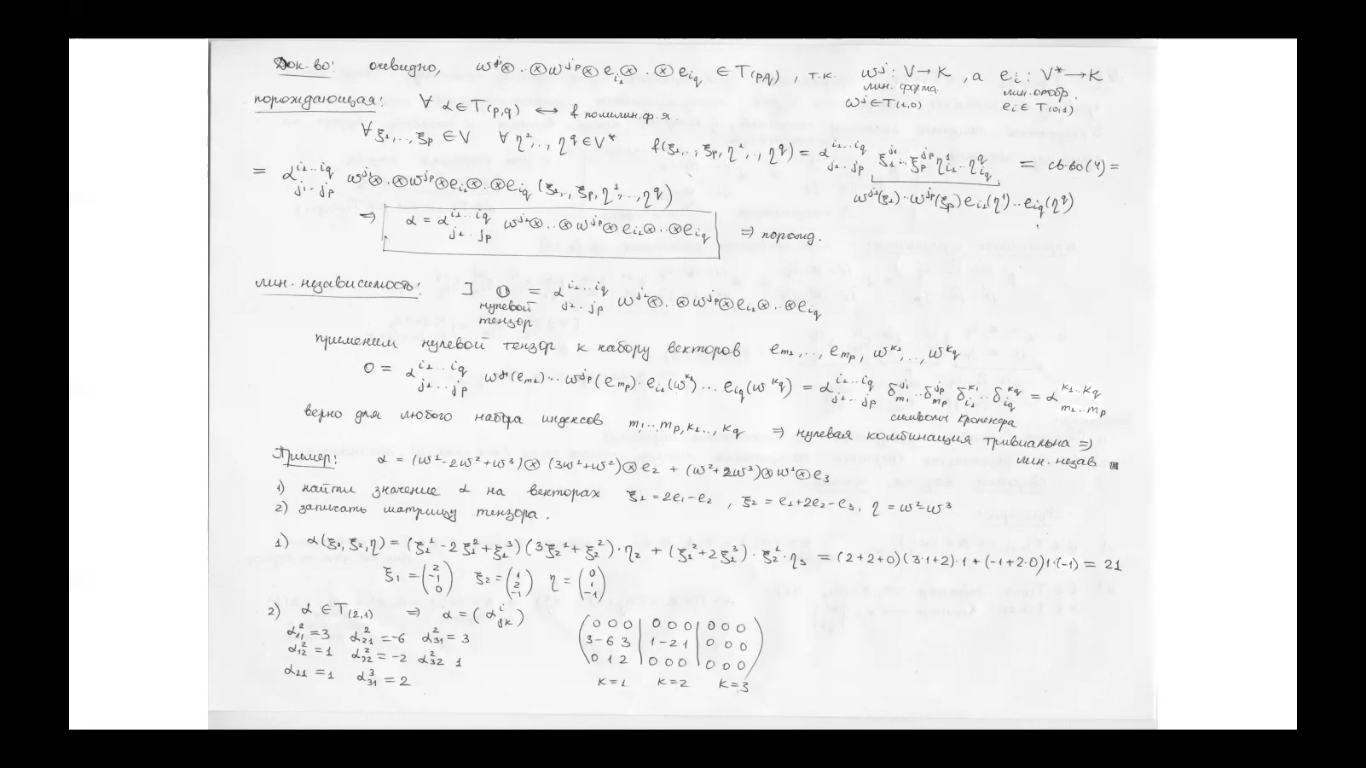
\includegraphics[height=\textheight * 10 / 21, width=\textwidth]{8_3-4}	
		\newline
		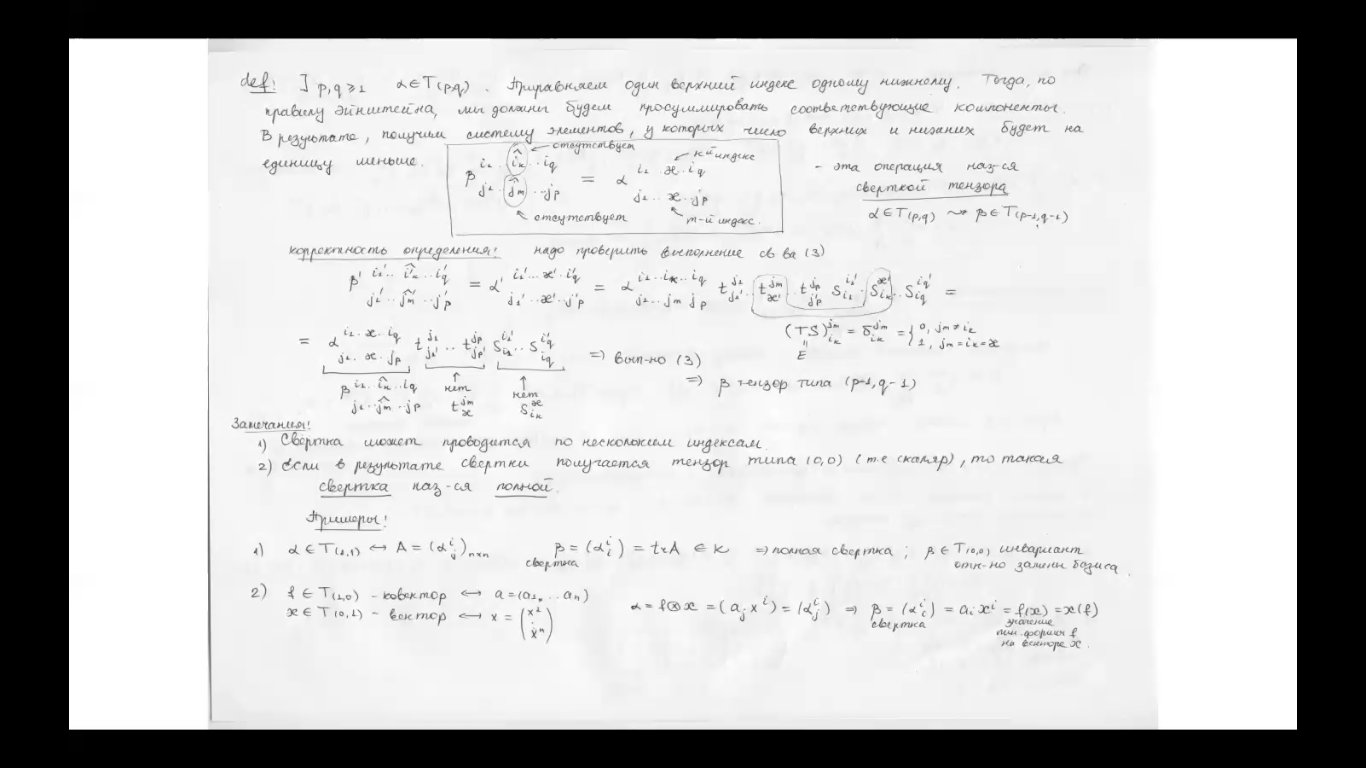
\includegraphics[height=\textheight * 10 / 21, width=\textwidth]{8_3-5}	
		\newline
		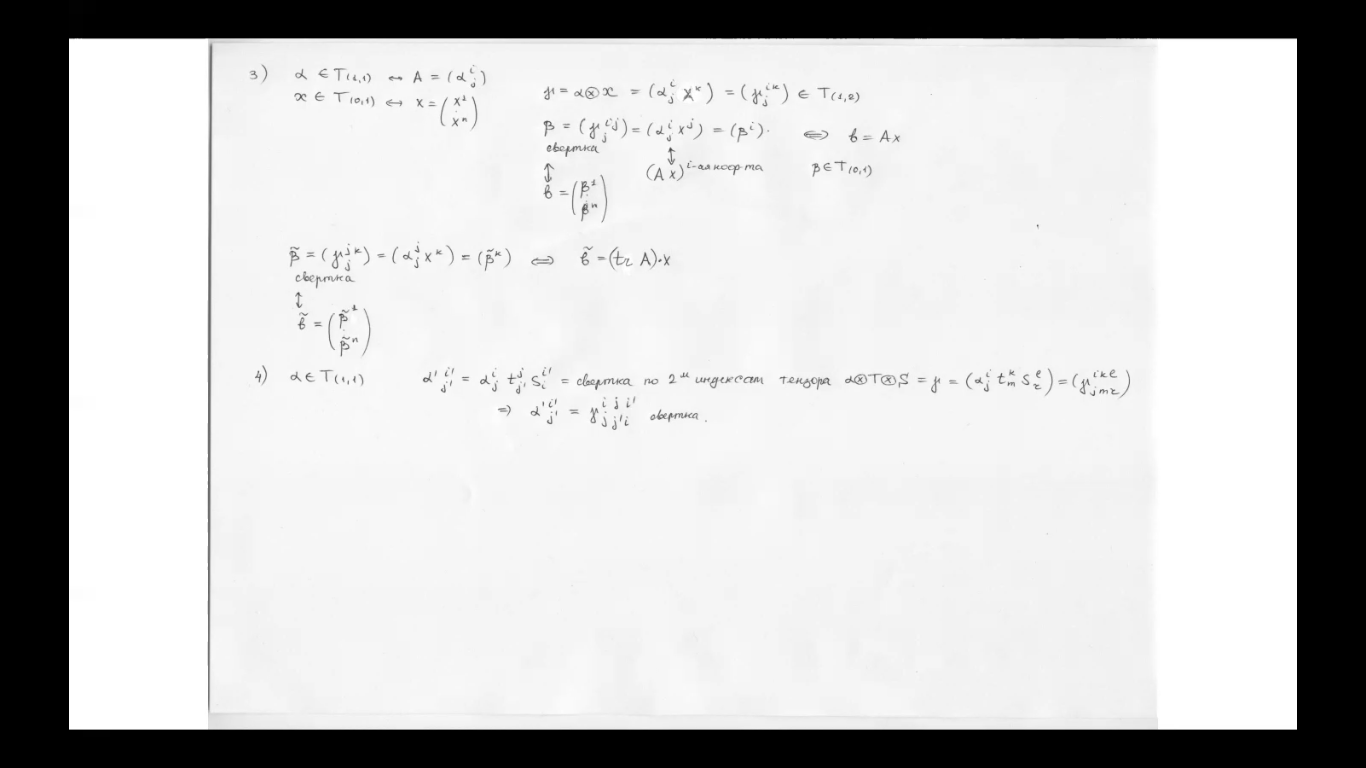
\includegraphics[height=\textheight * 10 / 21, width=\textwidth]{8_3-6}	
		\newline			
		
		
	\subsection{Транспонирование тензора. Симметрические и кососимметричческие тензоры.}
	 	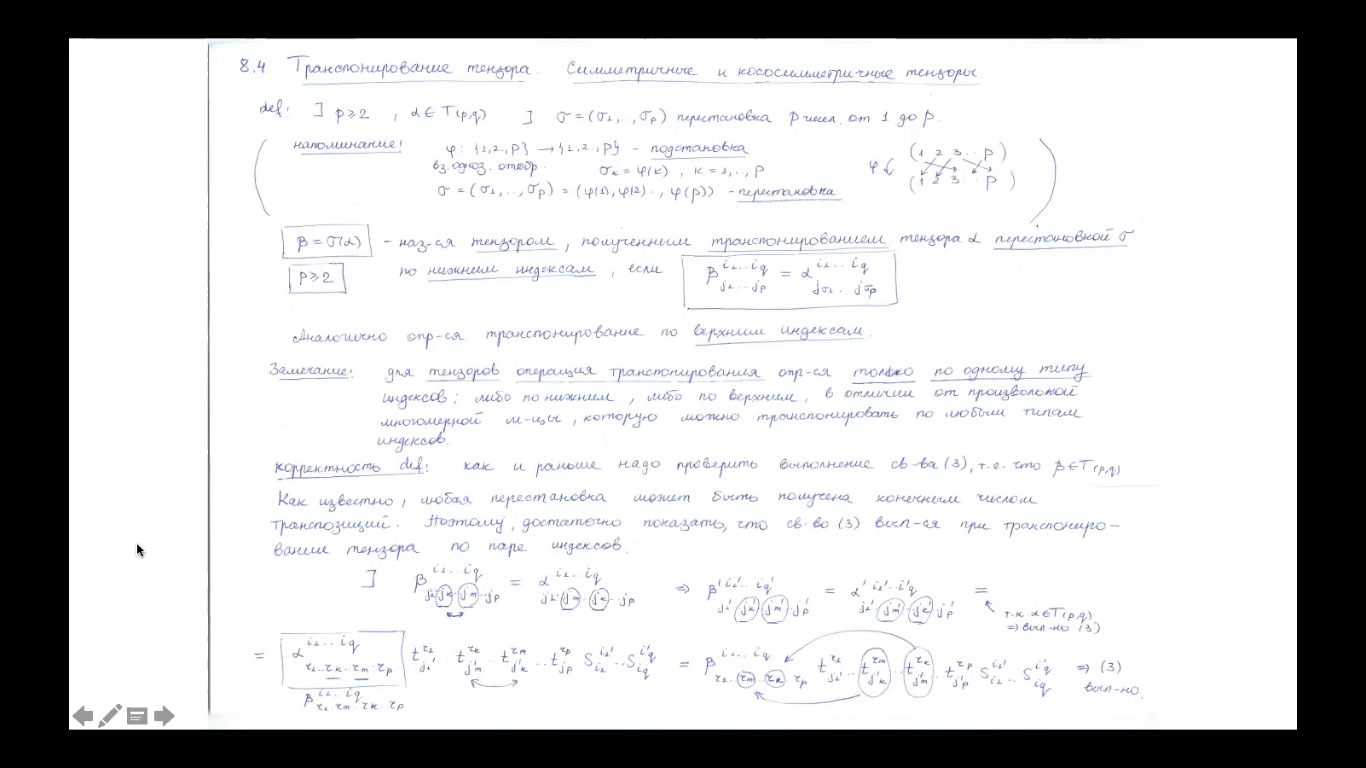
\includegraphics[height=\textheight * 10 / 21, width=\textwidth]{8_4-1}	
		\newline
		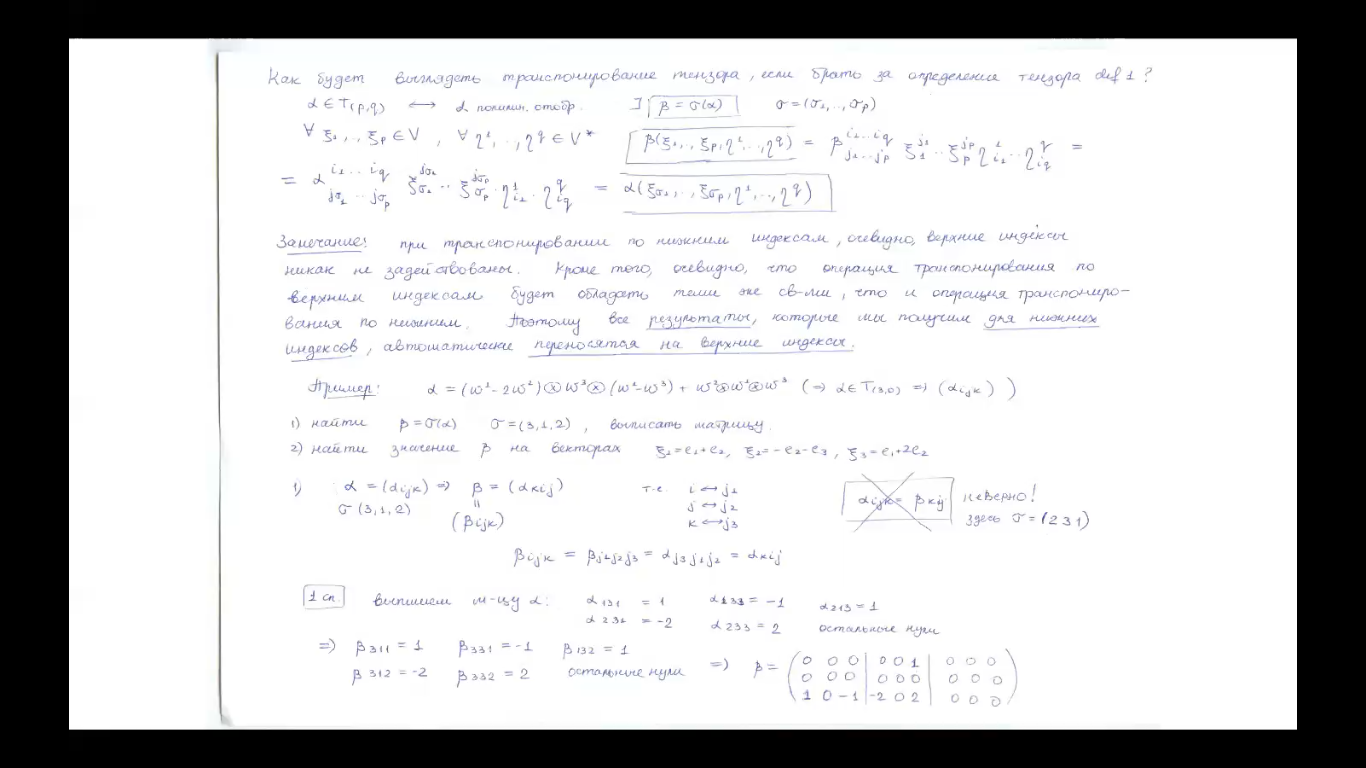
\includegraphics[height=\textheight * 10 / 21, width=\textwidth]{8_4-2}	
		\newline
		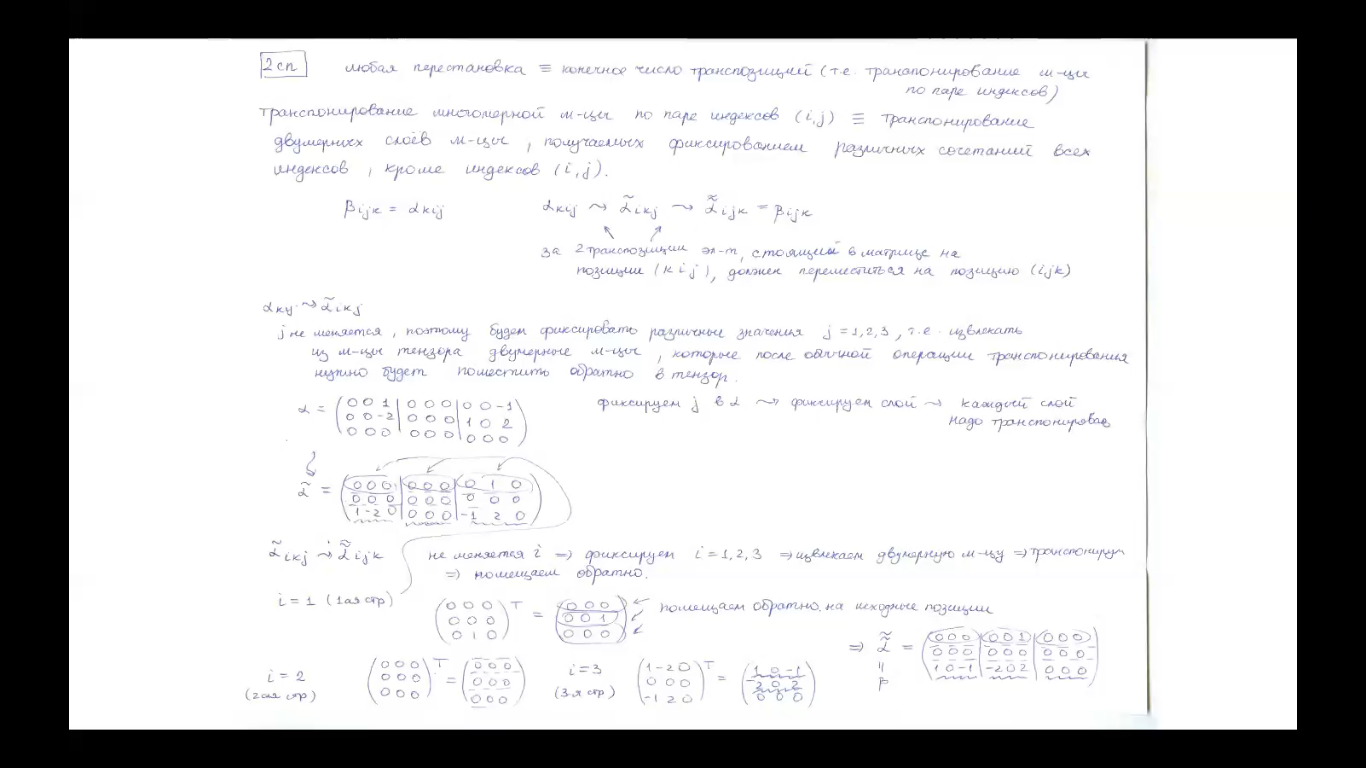
\includegraphics[height=\textheight * 10 / 21, width=\textwidth]{8_4-3}	
		\newline
		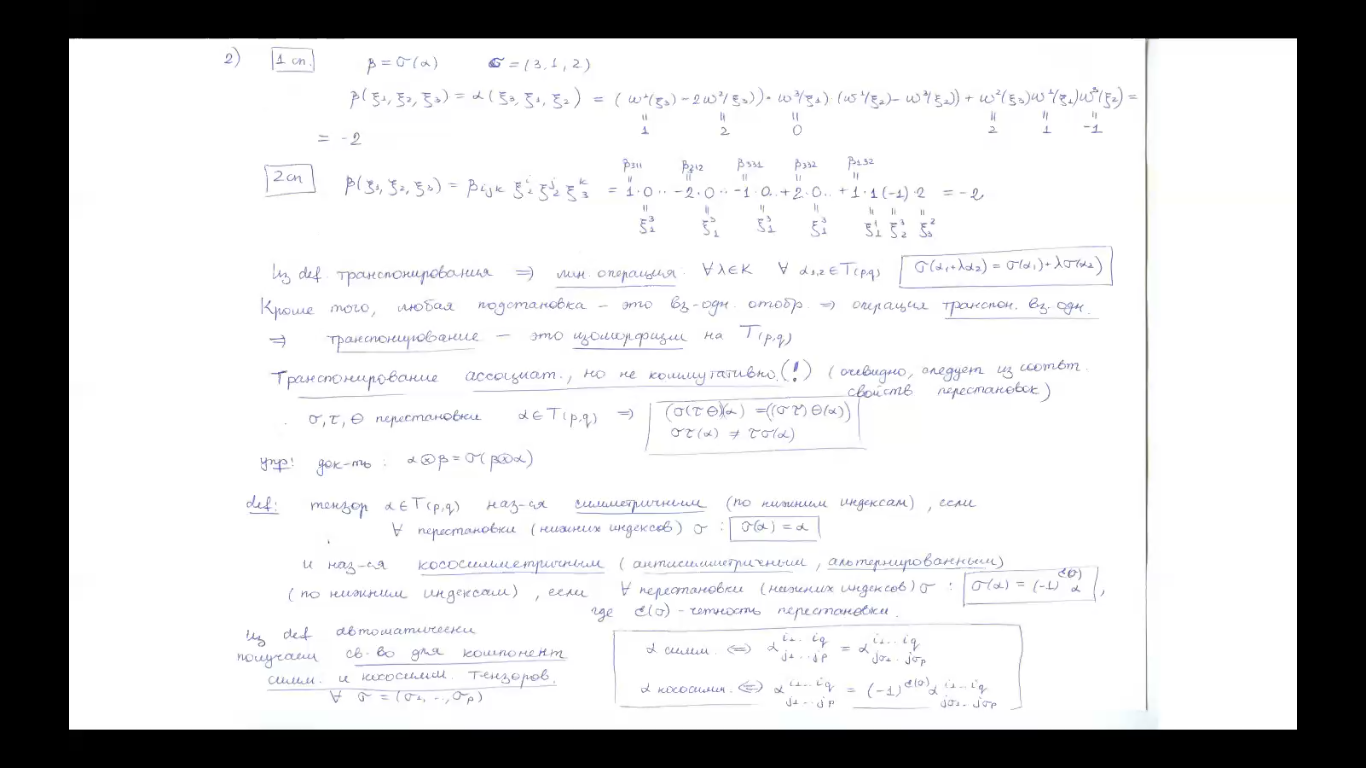
\includegraphics[height=\textheight * 10 / 21, width=\textwidth]{8_4-4}	
		\newline
		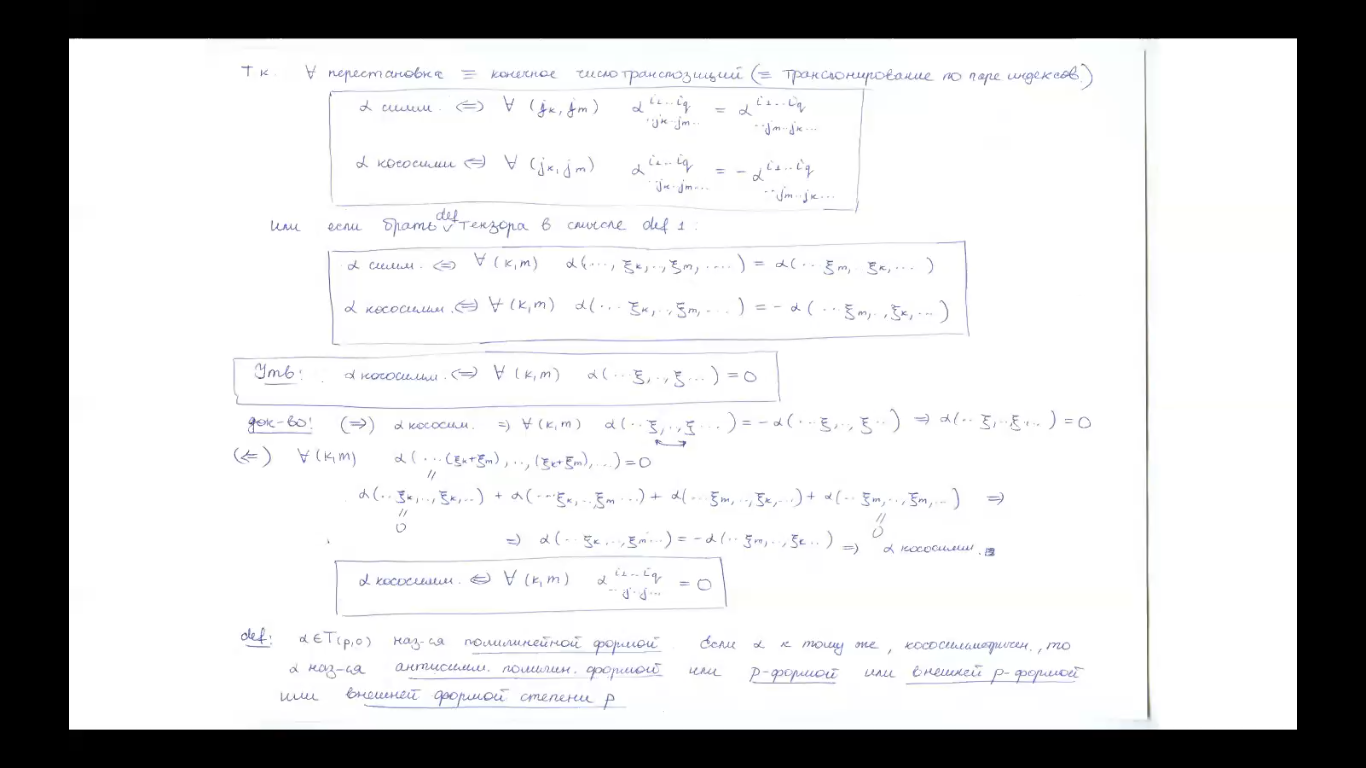
\includegraphics[height=\textheight * 10 / 21, width=\textwidth]{8_4-5}	
		\newline
		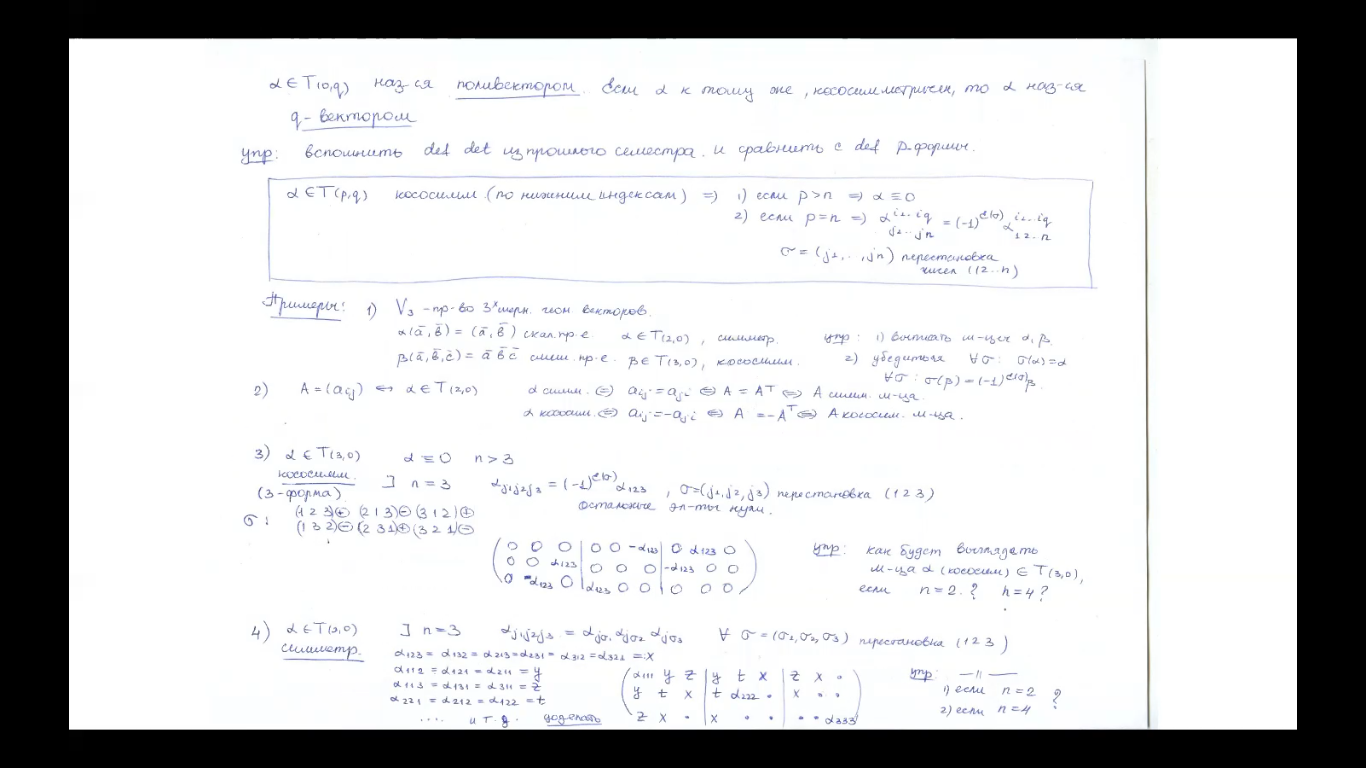
\includegraphics[height=\textheight * 10 / 21, width=\textwidth]{8_4-6}	
		\newline			
		
		
	\subsection{Операции альтернирования и симметрирования тензоров}
	 	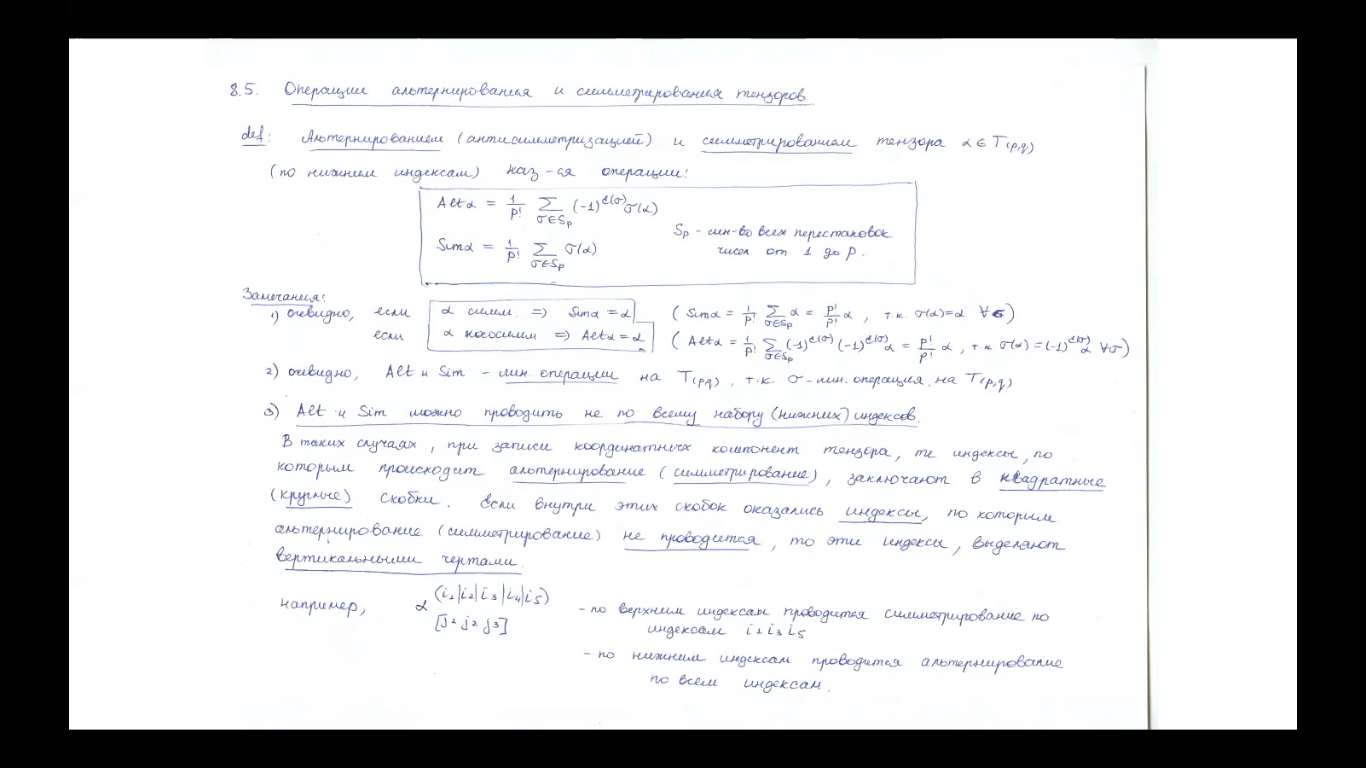
\includegraphics[height=\textheight * 10 / 21, width=\textwidth]{8_5-1}	
		\newline
		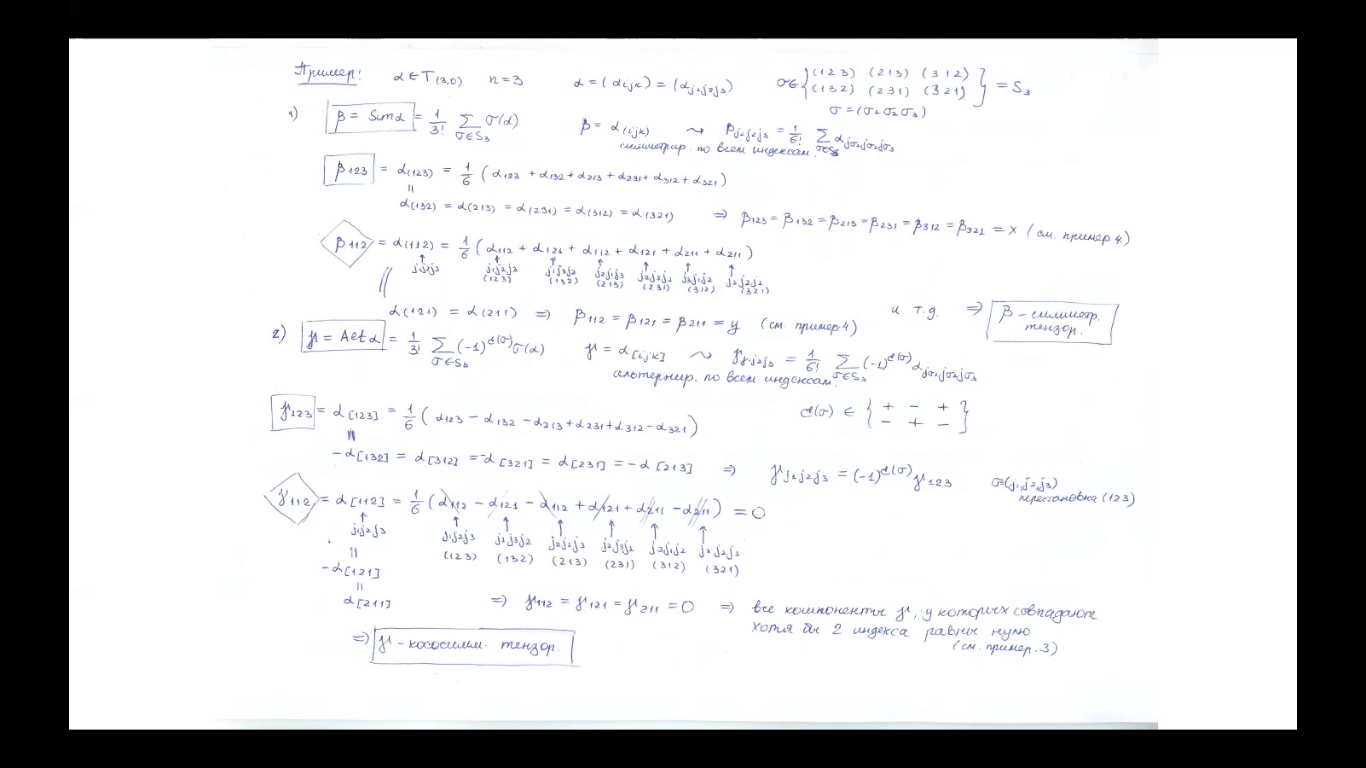
\includegraphics[height=\textheight * 10 / 21, width=\textwidth]{8_5-2}	
		\newline
		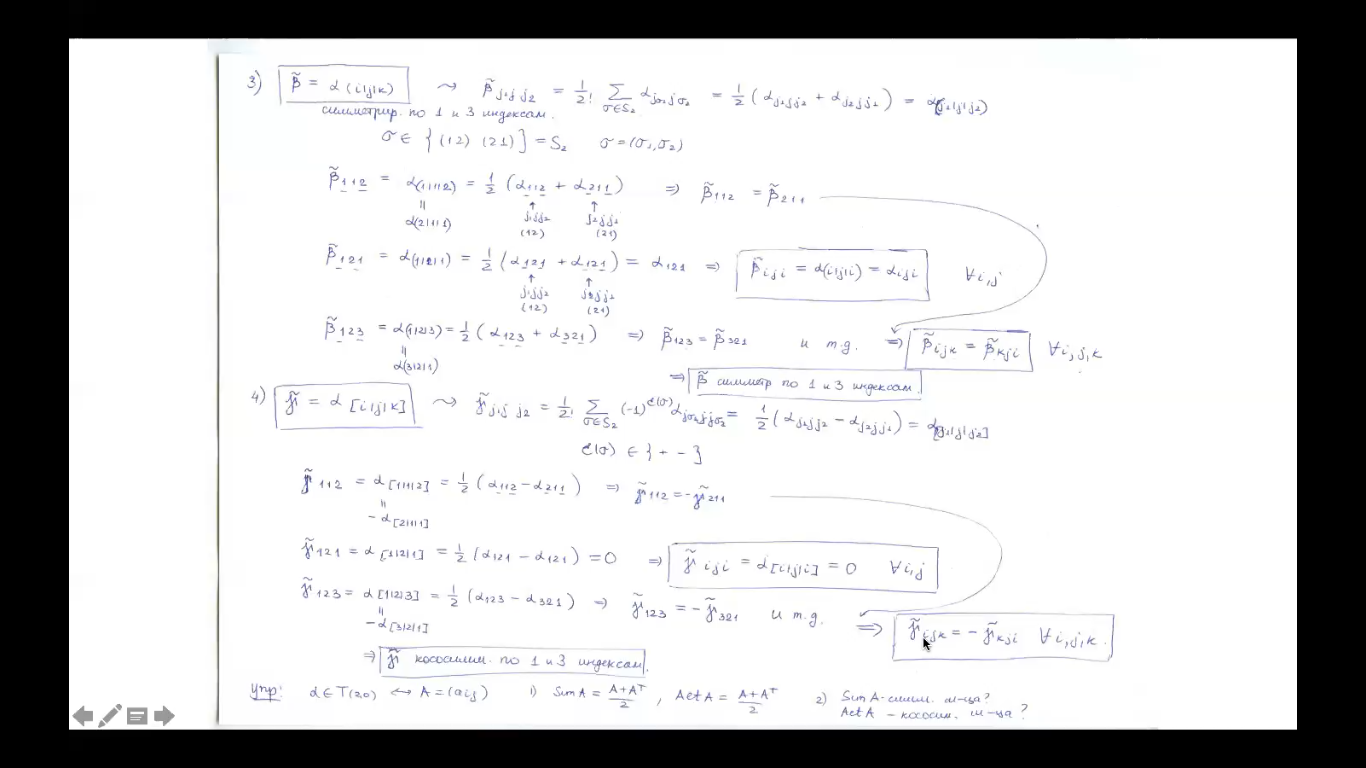
\includegraphics[height=\textheight * 10 / 21, width=\textwidth]{8_5-3}	
		\newline\end{document}